\documentclass[handout]{beamer}

\usepackage{fontspec} 
% \usepackage{lsp-makros}
\useoutertheme{lsp}

\usepackage{lsptitle}
\usepackage{url}
\def\two@digits#1{\ifnum#1<10 0\fi\number#1}
\def\mytoday{\two@digits{\number\day}.\two@digits{\number\month}.\number\year}


\usepackage{xspace,multicol}
\newcommand{\latex}{\LaTeX\xspace}
\usepackage{tikz}


\newcounter{lastpagemainpart}
\footnotesep0pt
\renewcommand{\footnoterule}{}
\usefootnotetemplate{
  \noindent
  \insertfootnotemark\insertfootnotetext}

\let\beamerfn=\footnote
\renewcommand{\footnote}[1]{%
\let\oldfnsize=\footnotesize%
\let\footnotesize=\tiny%
\beamerfn<\thebeamerpauses->{#1}%
\let\footnotesize=\oldfnsize}


\date{\today}

\usepackage{eurosym}  
 
\renewcommand{\centerline}[1]{\hfill#1\hfill\hfill\mbox{}}


\title{\mbox{Shopping around for examples:} \mbox{faceted browsing of linguistic} literature Amazon™ style}
% \institute{FU Berlin}
\author[Nordhoff]{Sebastian Nordhoff}



\begin{document}
\lspbeamertitle

\section{Use case}

\frame{
\frametitle{Use case: Shopping around\newline for examples}
\begin{itemize}
 \item Sometimes, a key example is needed to prove a certain point
 \item That example must combine two or more categories
  \begin{itemize}
  \item \textsc{past} + \textsc{erg} vs. \textsc{fut} + \textsc{erg}
  \item \textsc{2pl} + \textsc{refl} 
  \item negation + complex sentence
  \item quotatives + interjection
  \end{itemize} 
  \item grammatical descriptions might describe each relevant feature, but not the combinations thereof
  \item example sentences can be a good proxy to retrieve passages of GDs which are relevant for the research question
  \item Make cherry-picking easier!
\end{itemize}
}

\section{Background}

 
\frame{
\frametitle{Exbase}
  \begin{itemize}
    \item developed from 2012-2015
    \item Exploratory approach, not analytical
    \item parsing of HH's grammmars
    \begin{itemize}
     \item Leipzig OCR version
    \end{itemize}
    \item  off-the shelf technology
    \item discontinued because of © problems, but resurrected for this workshop
    \item server not powerful enough, but will try a demo this afternoon 
\url{http://www.glottotopia.org/solr/exbase/browse?&fq=dtype\%3A\%22example\%22&q=&fq=words:\%5B10+TO+15\%7D\#}
  \end{itemize}
}





\section{Walkthrough}

\frame{
\frametitle{Walkthrough}
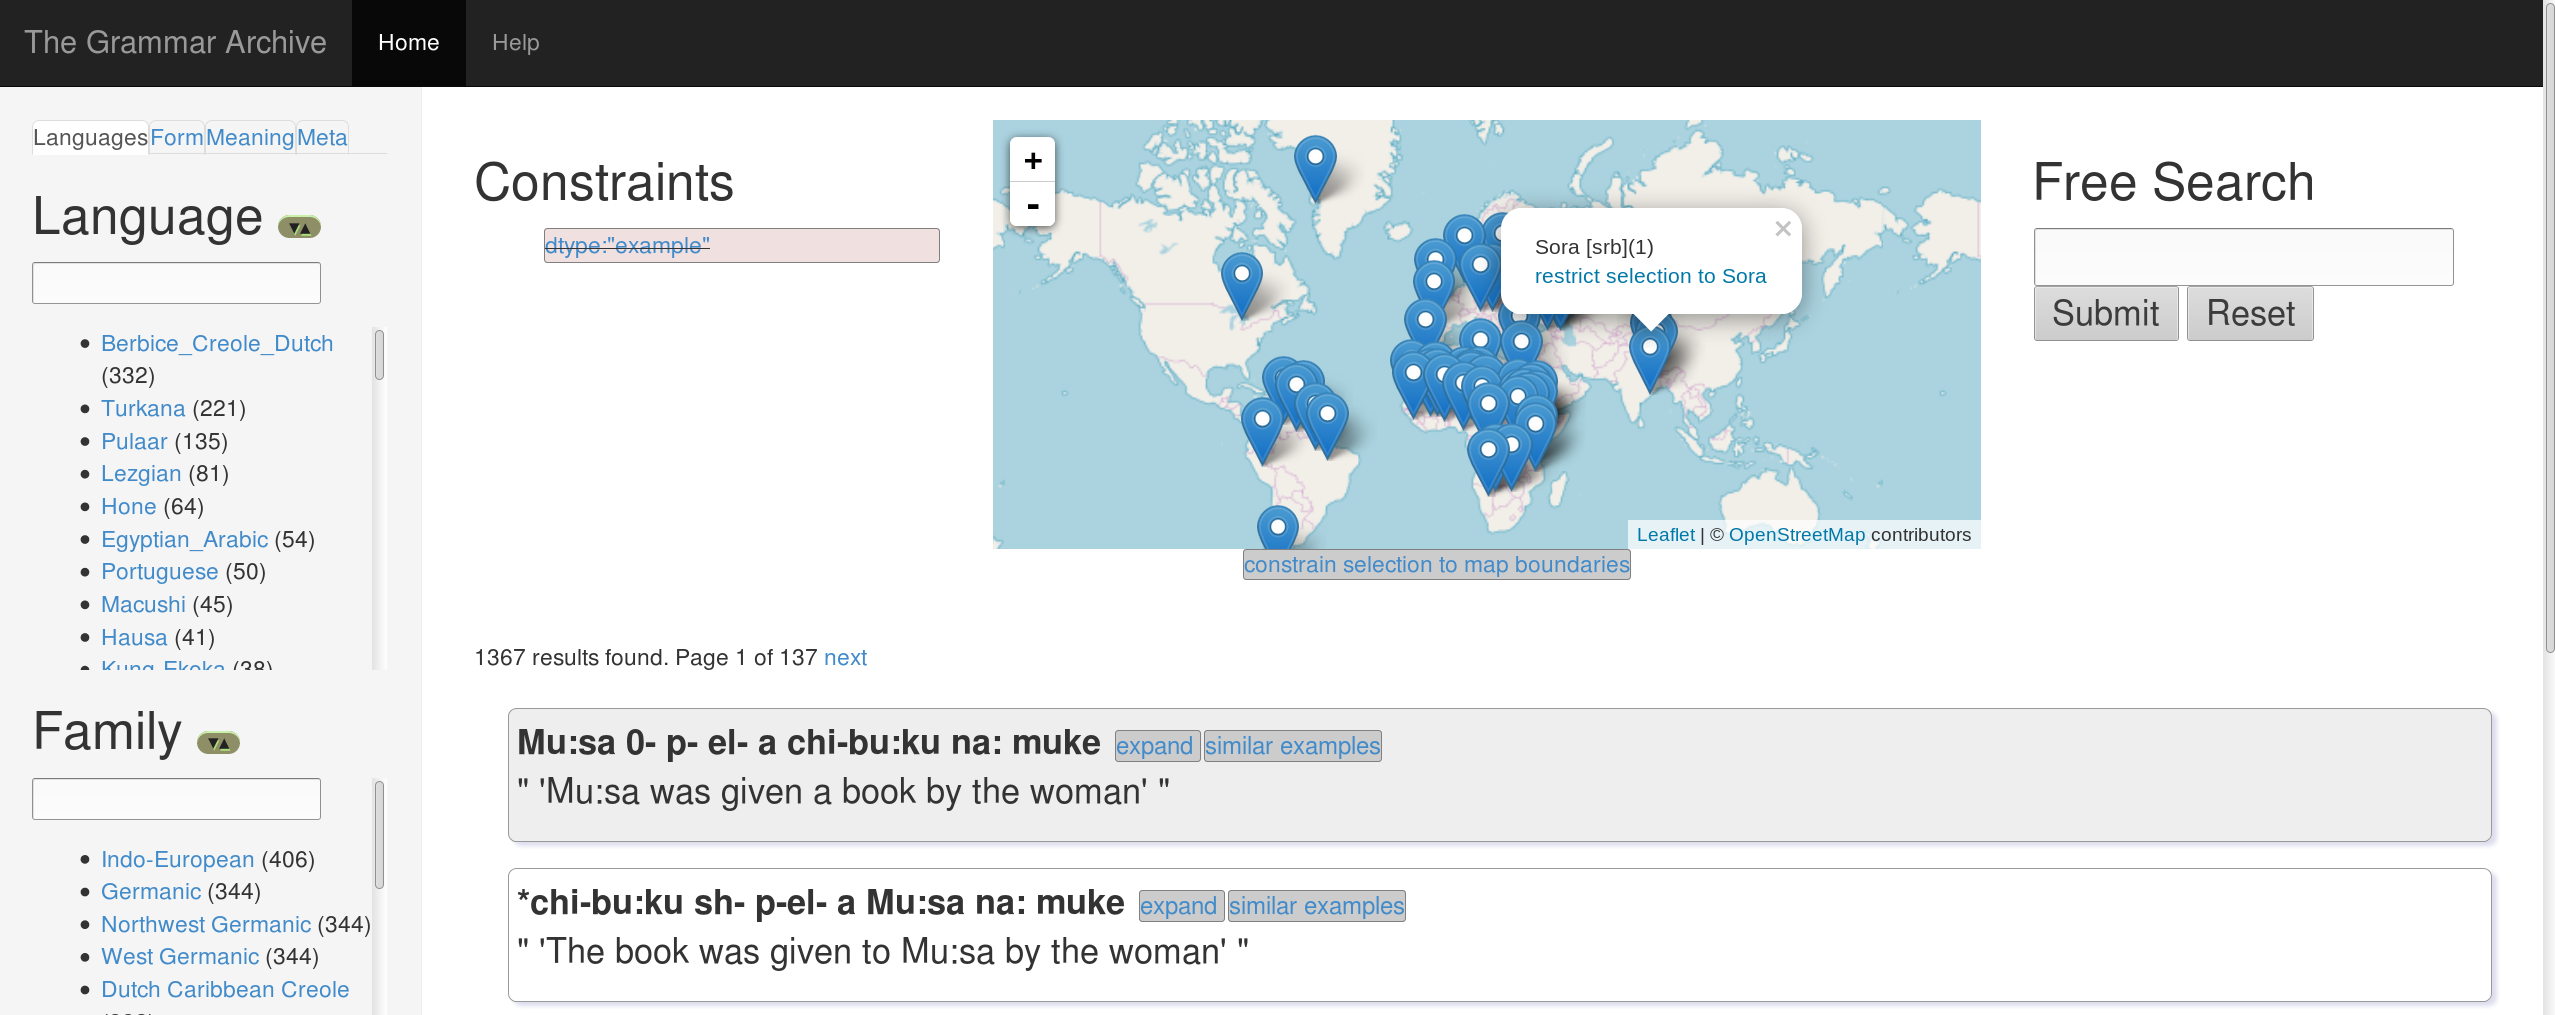
\includegraphics[width=\textwidth]{pics/overview.png} 
}

\frame{
\frametitle{Metadata constraints}
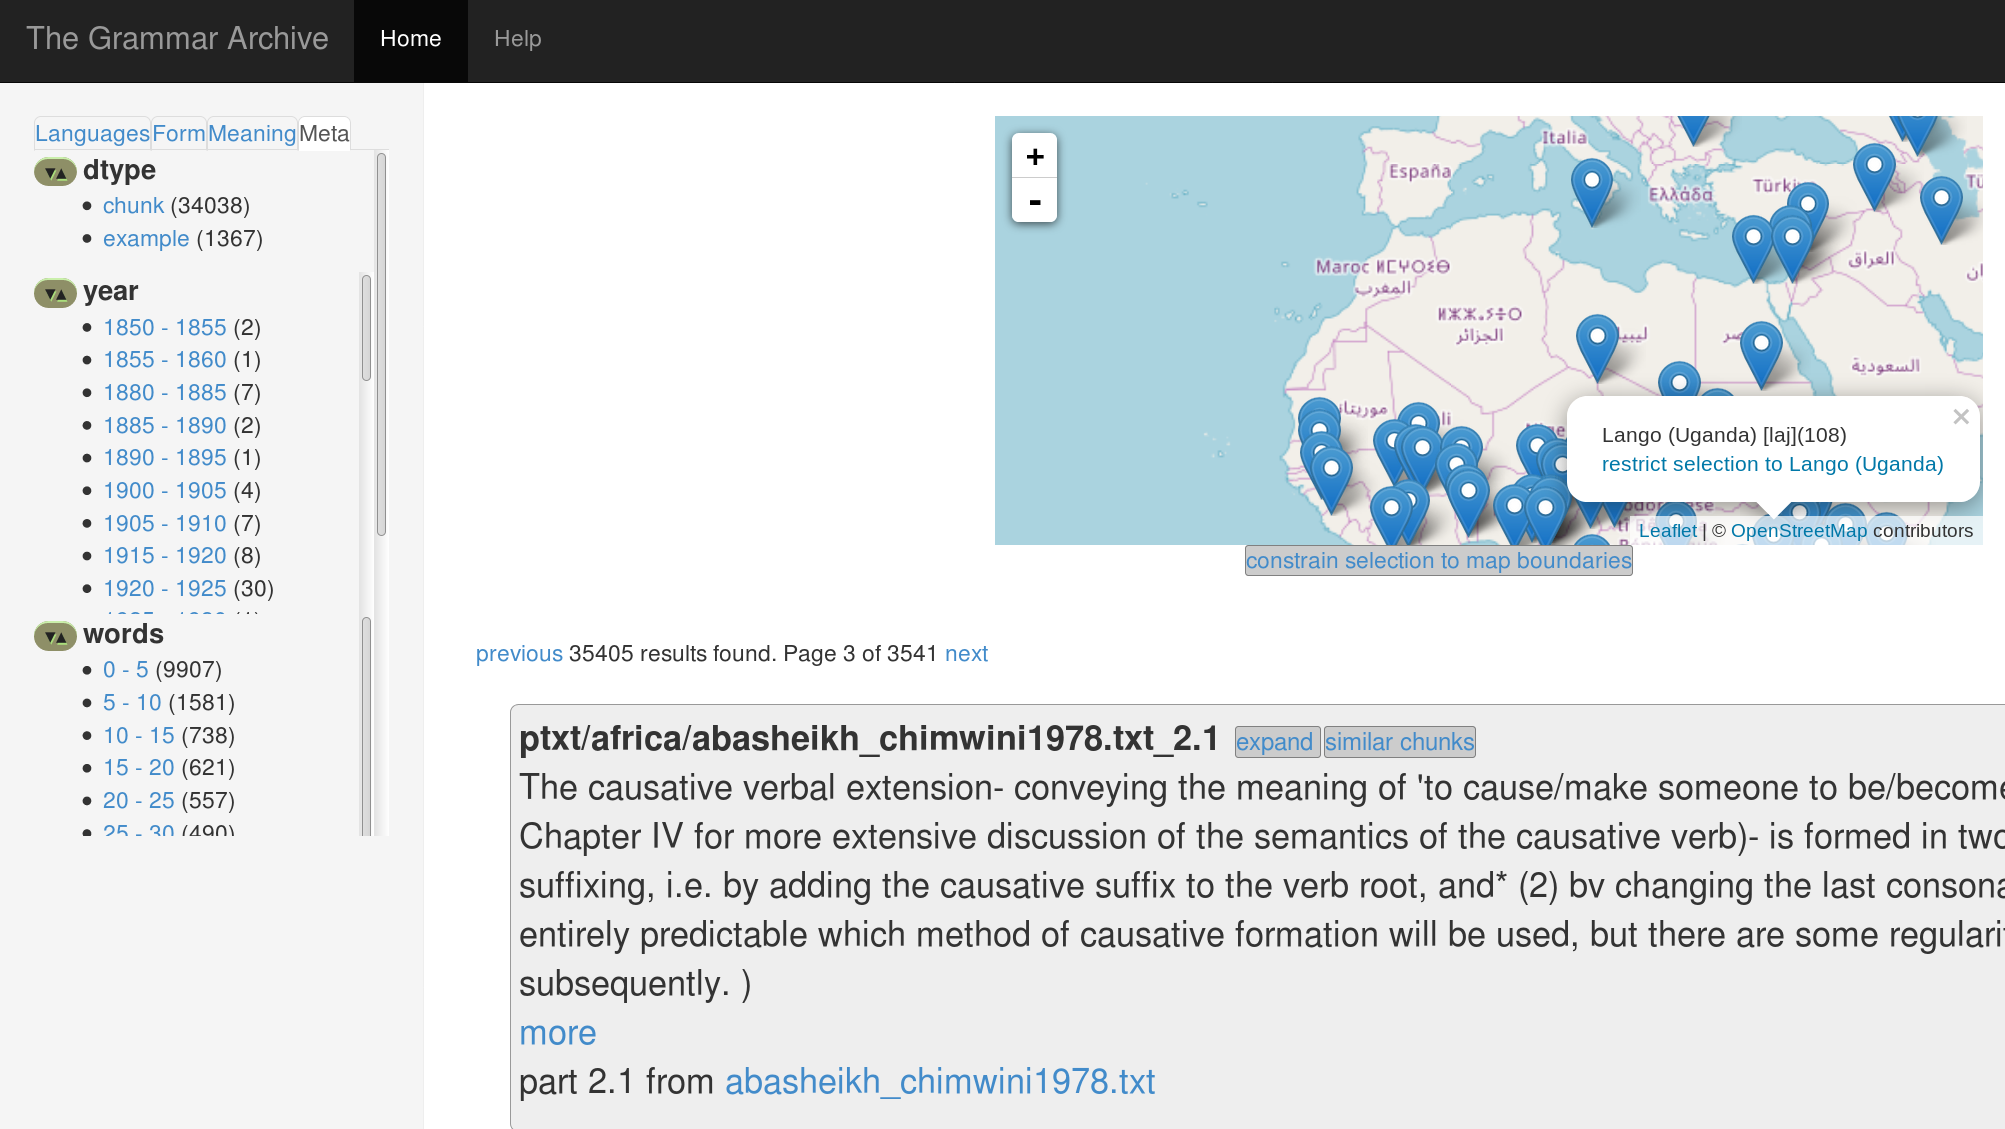
\includegraphics[height=\textheight]{pics/meta.png} 
}

% \frame{
% \frametitle{Example view}
% 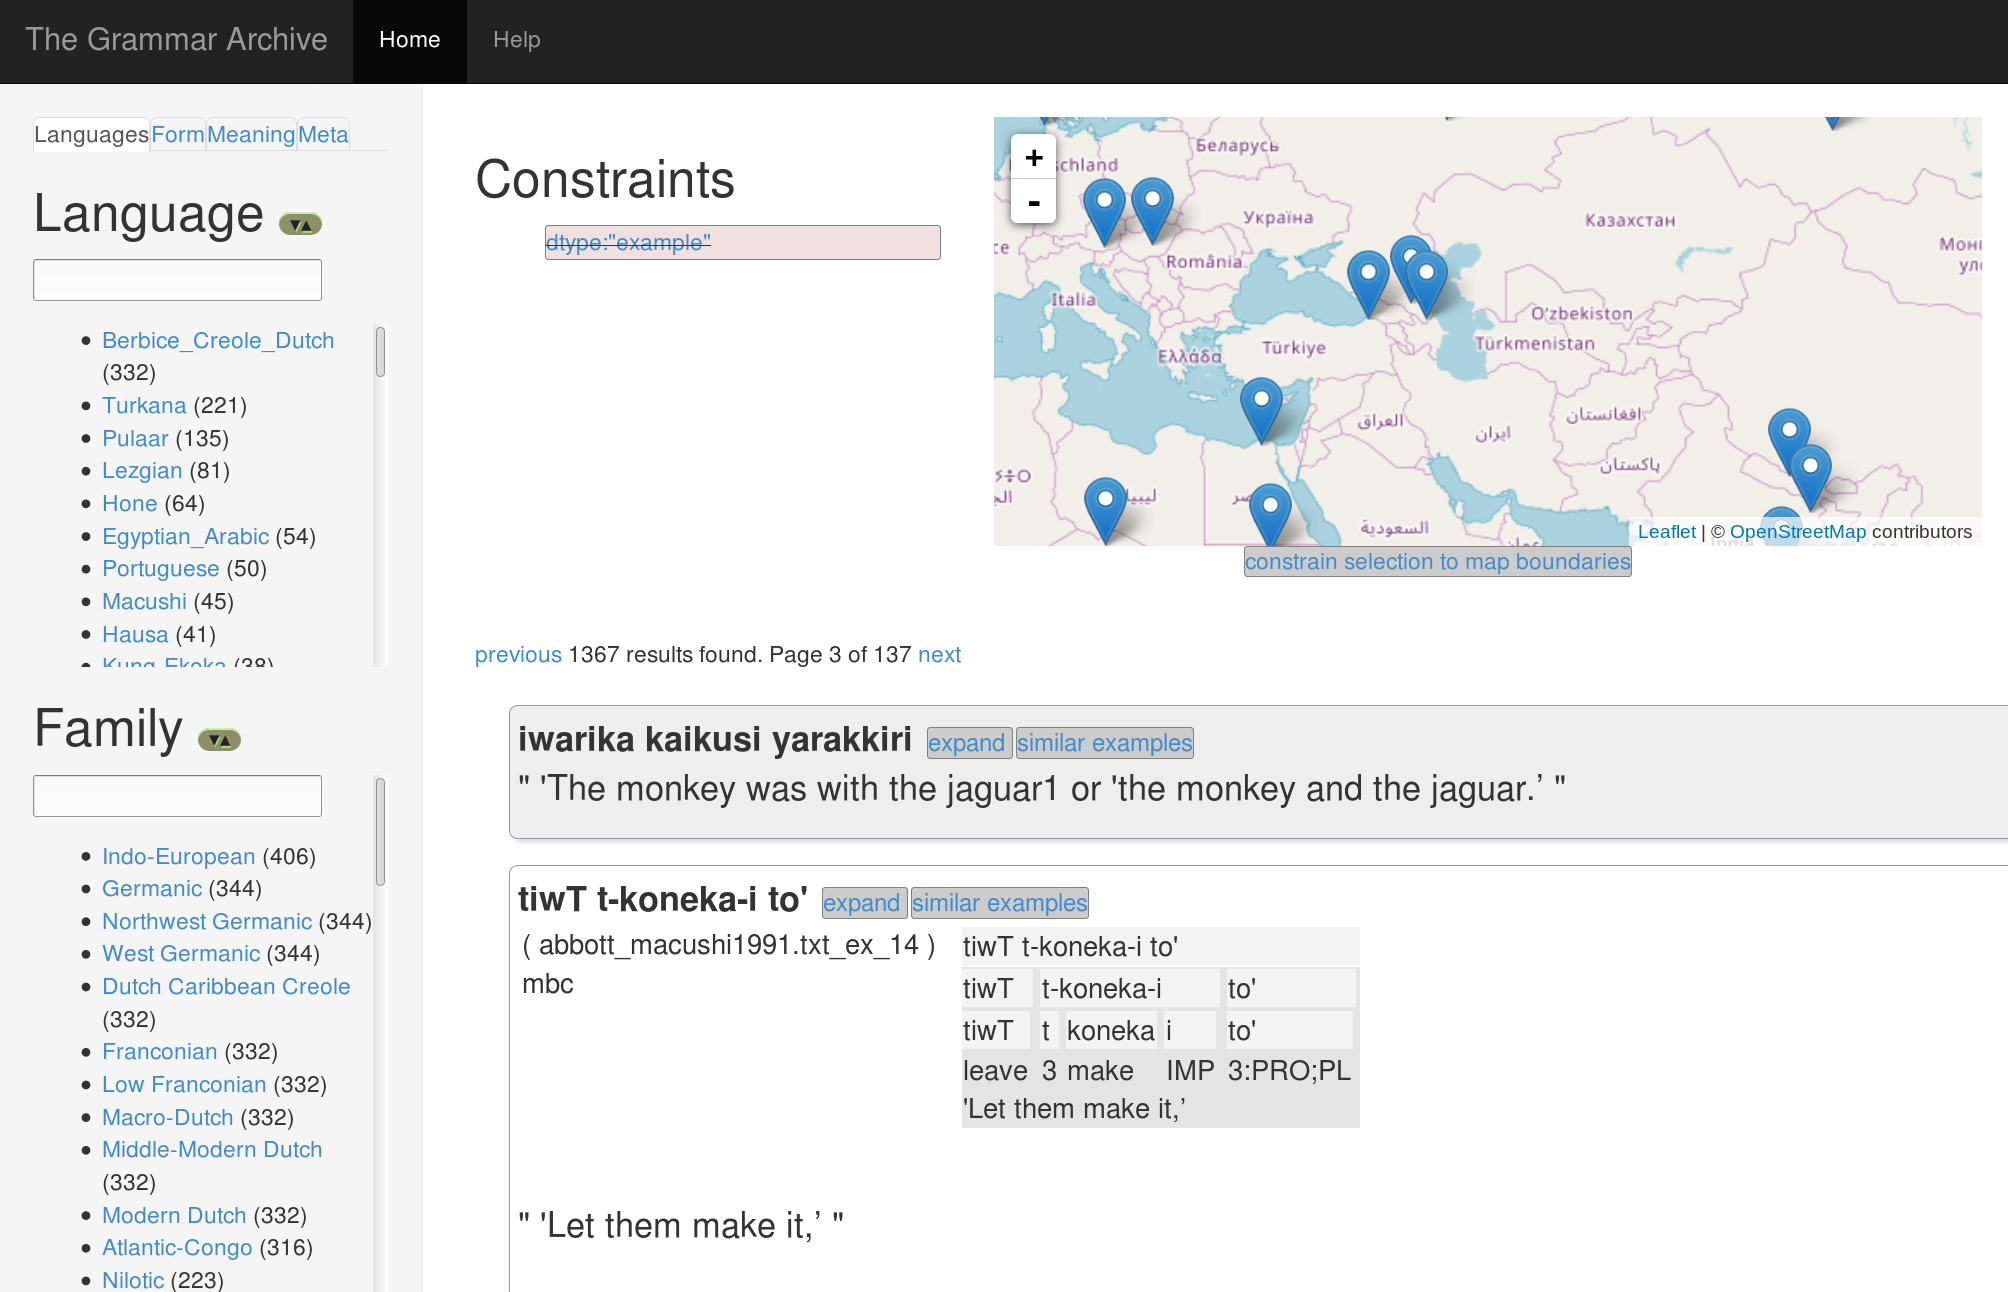
\includegraphics[height=\textheight]{pics/example-IMT.png} 
% }

\frame{
\frametitle{Search languages}
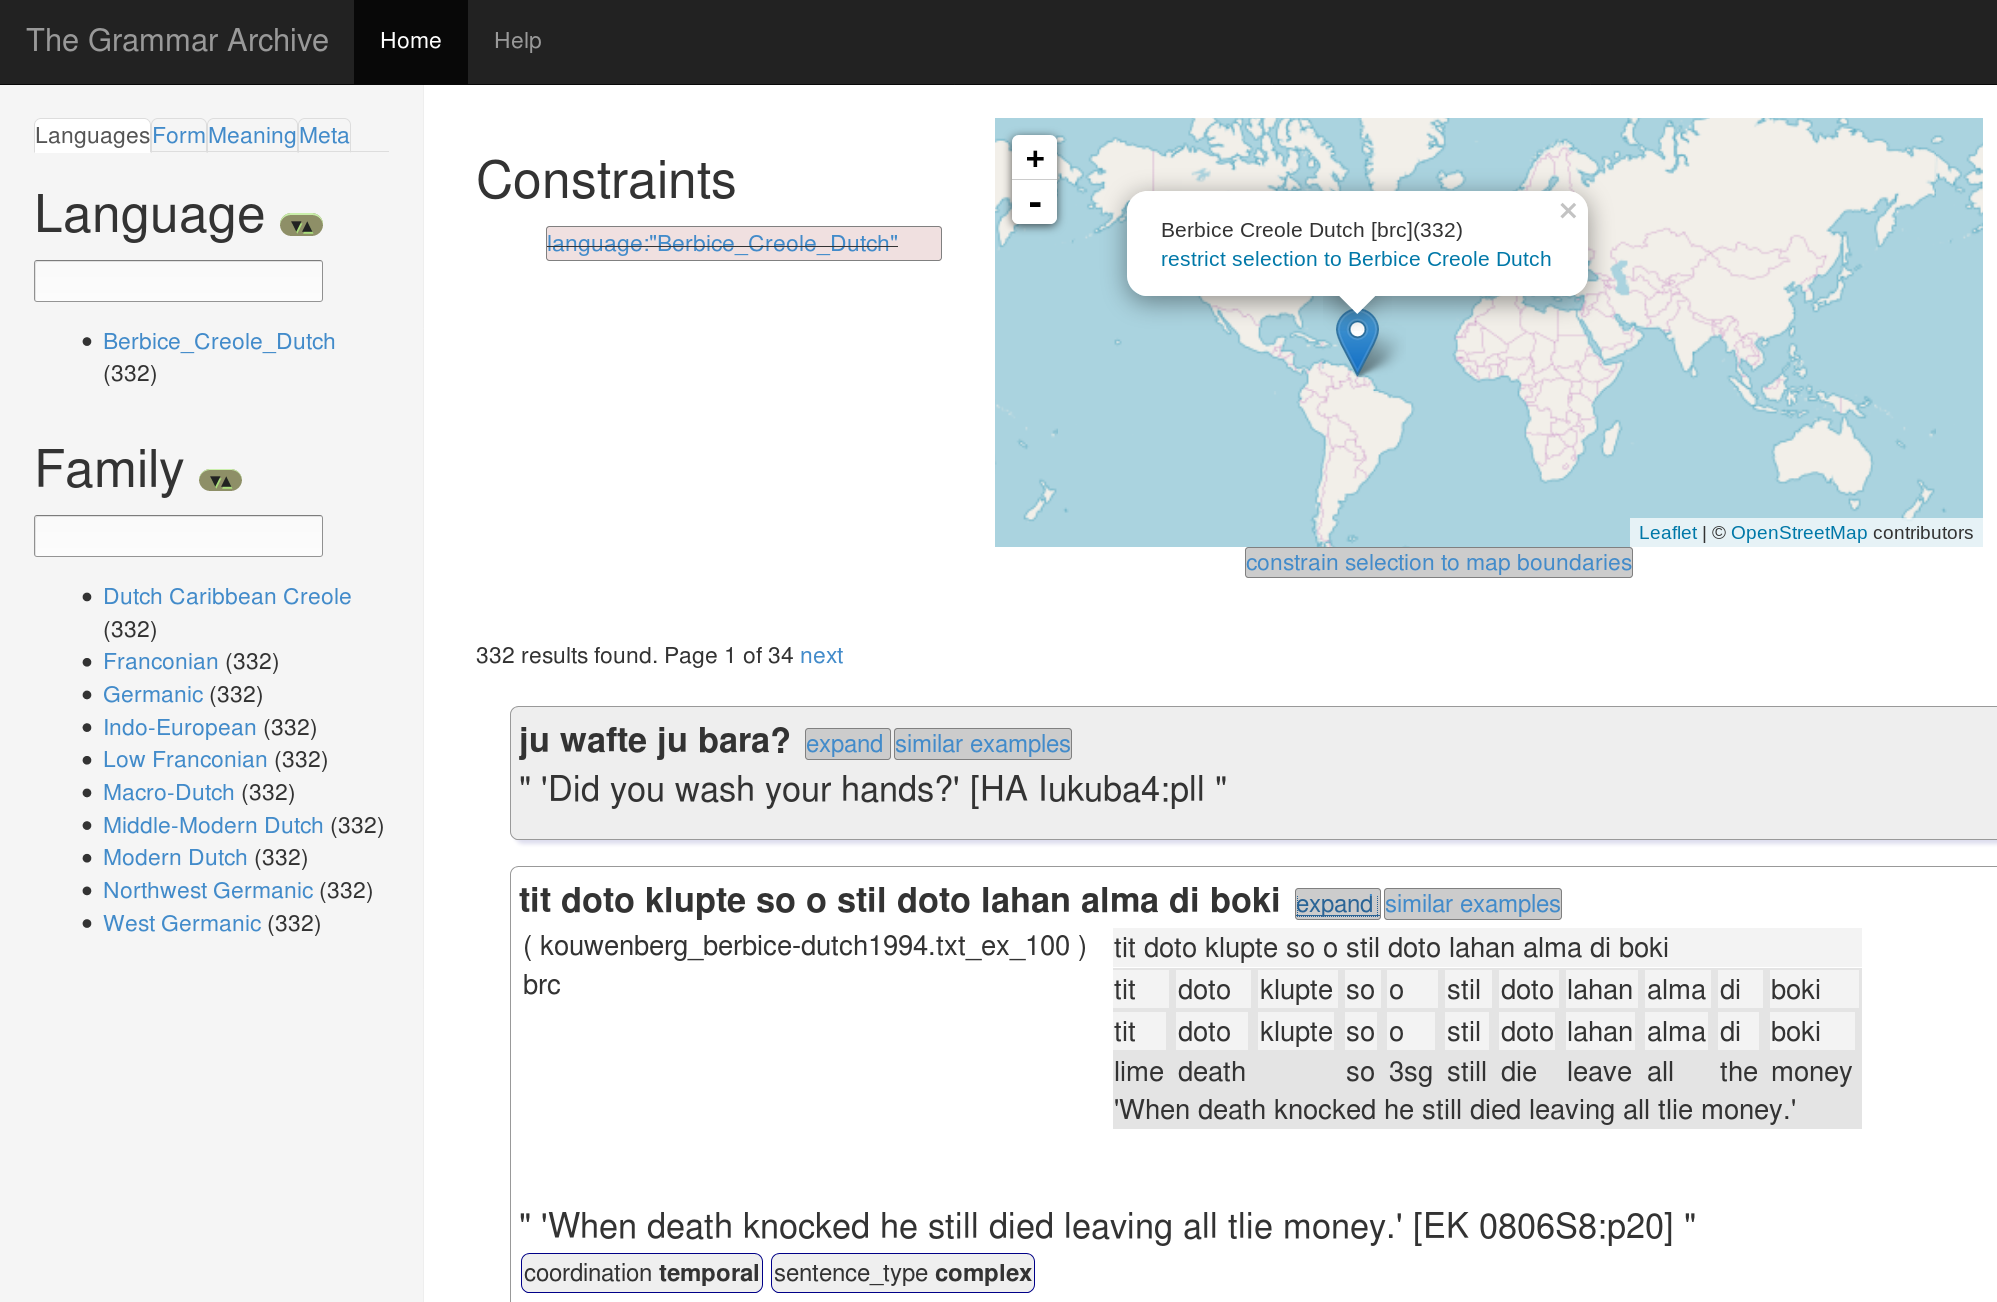
\includegraphics[height=\textheight]{pics/languagessearch.png} 
}

% \frame{
% \frametitle{Example view: tags}
% 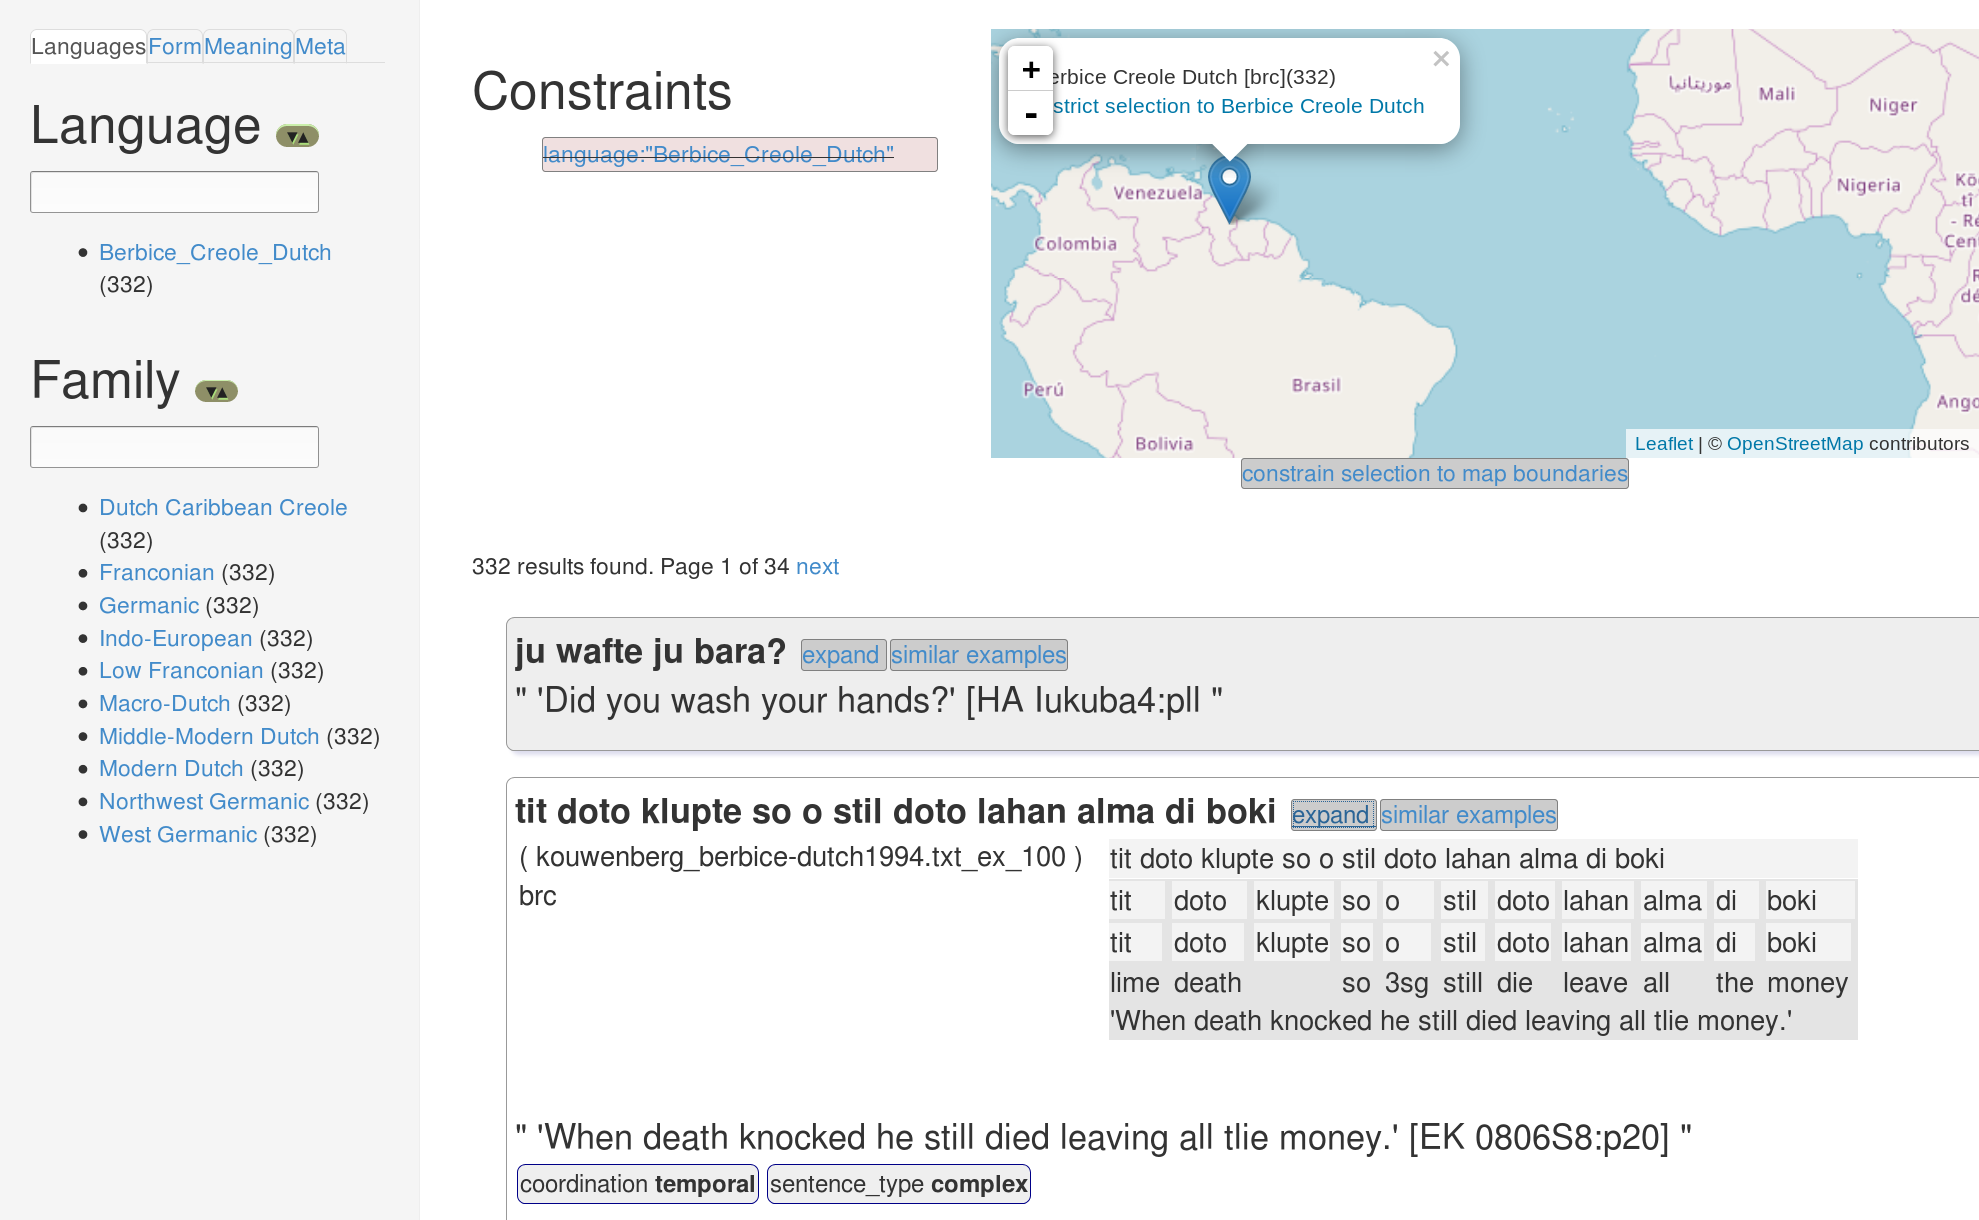
\includegraphics[height=\textheight]{pics/tags.png} 
% }



\frame{
\frametitle{Search for higher nodes (=families)}
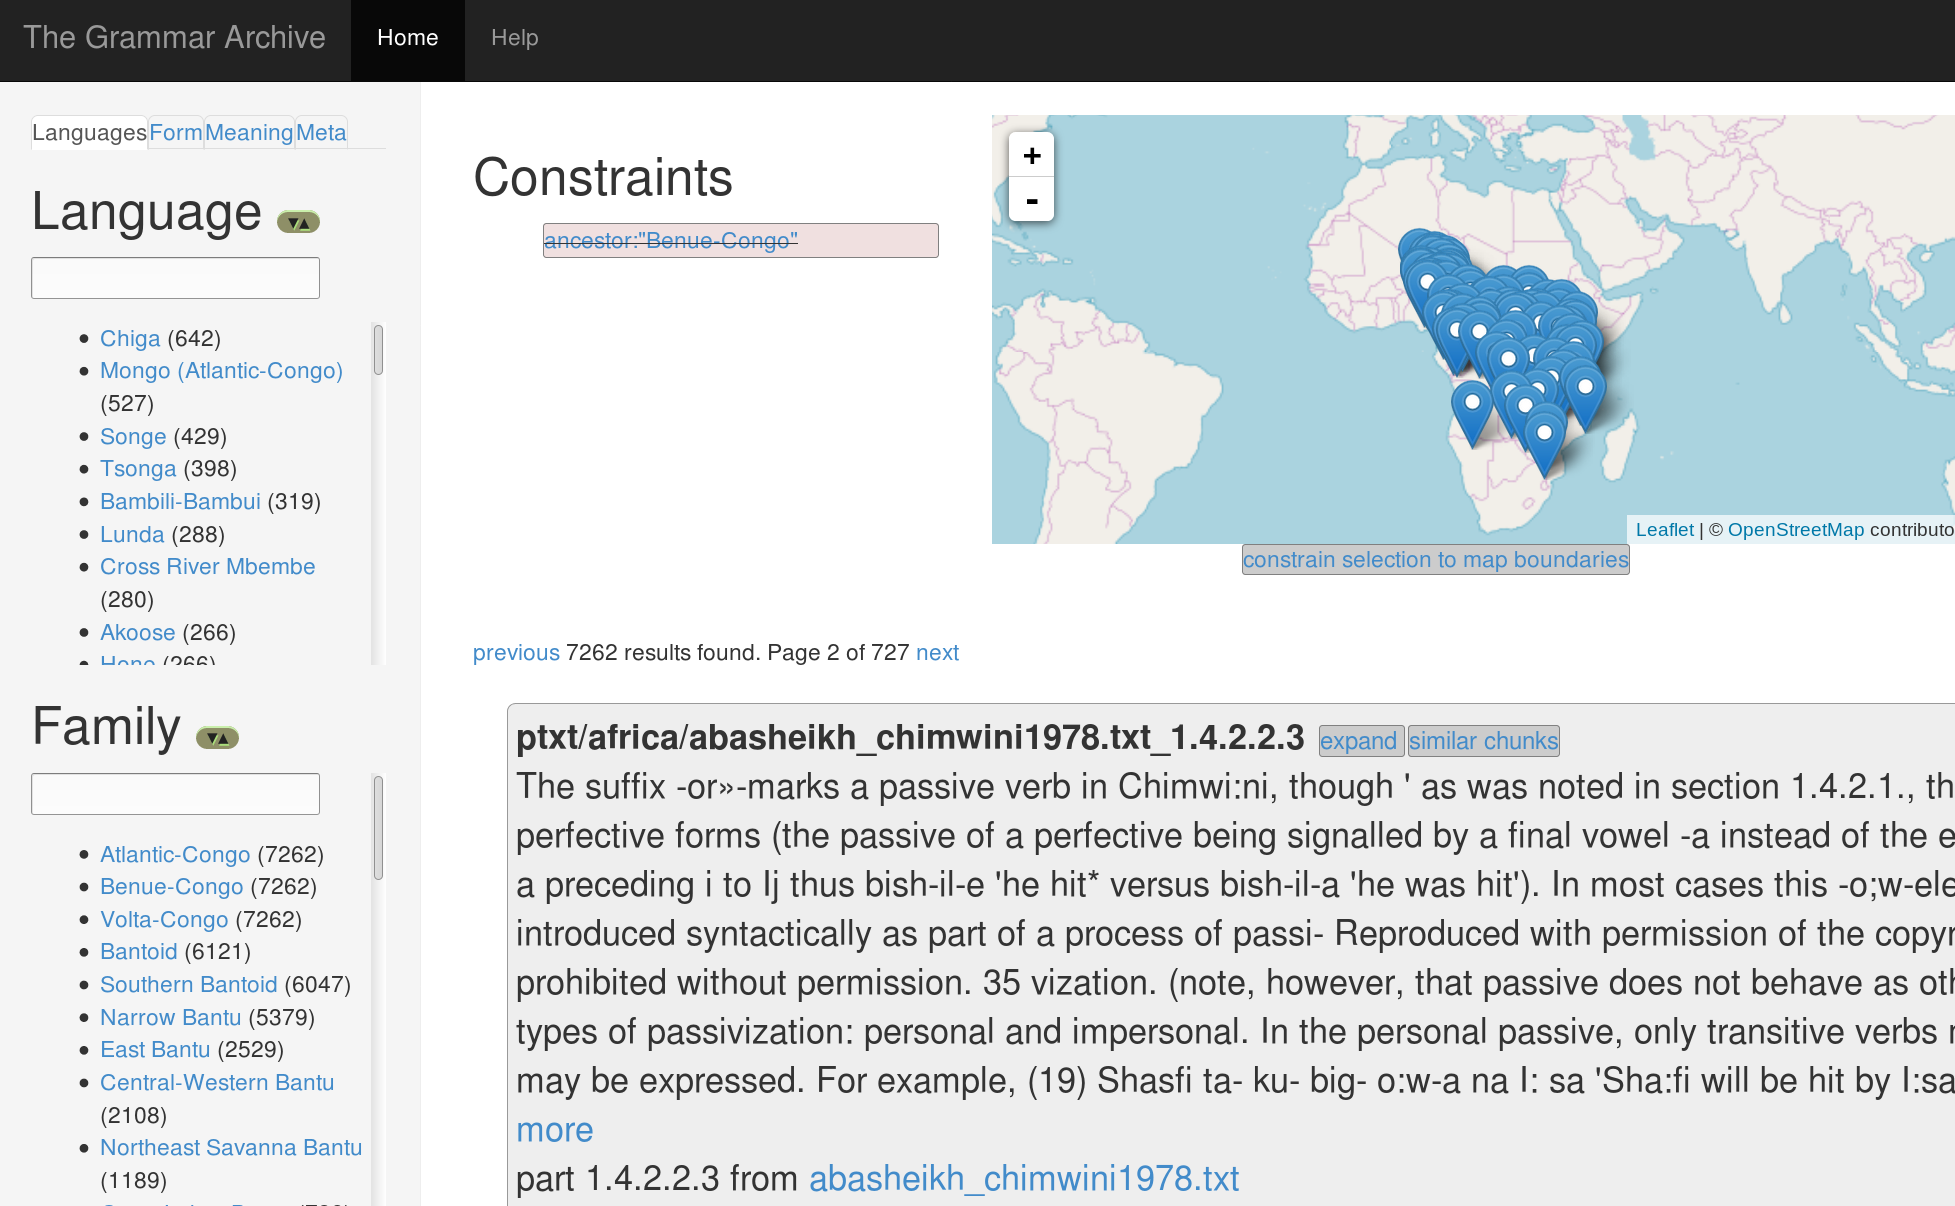
\includegraphics[height=\textheight]{pics/familysearch.png} 
}


\frame{
\frametitle{Geosearch}
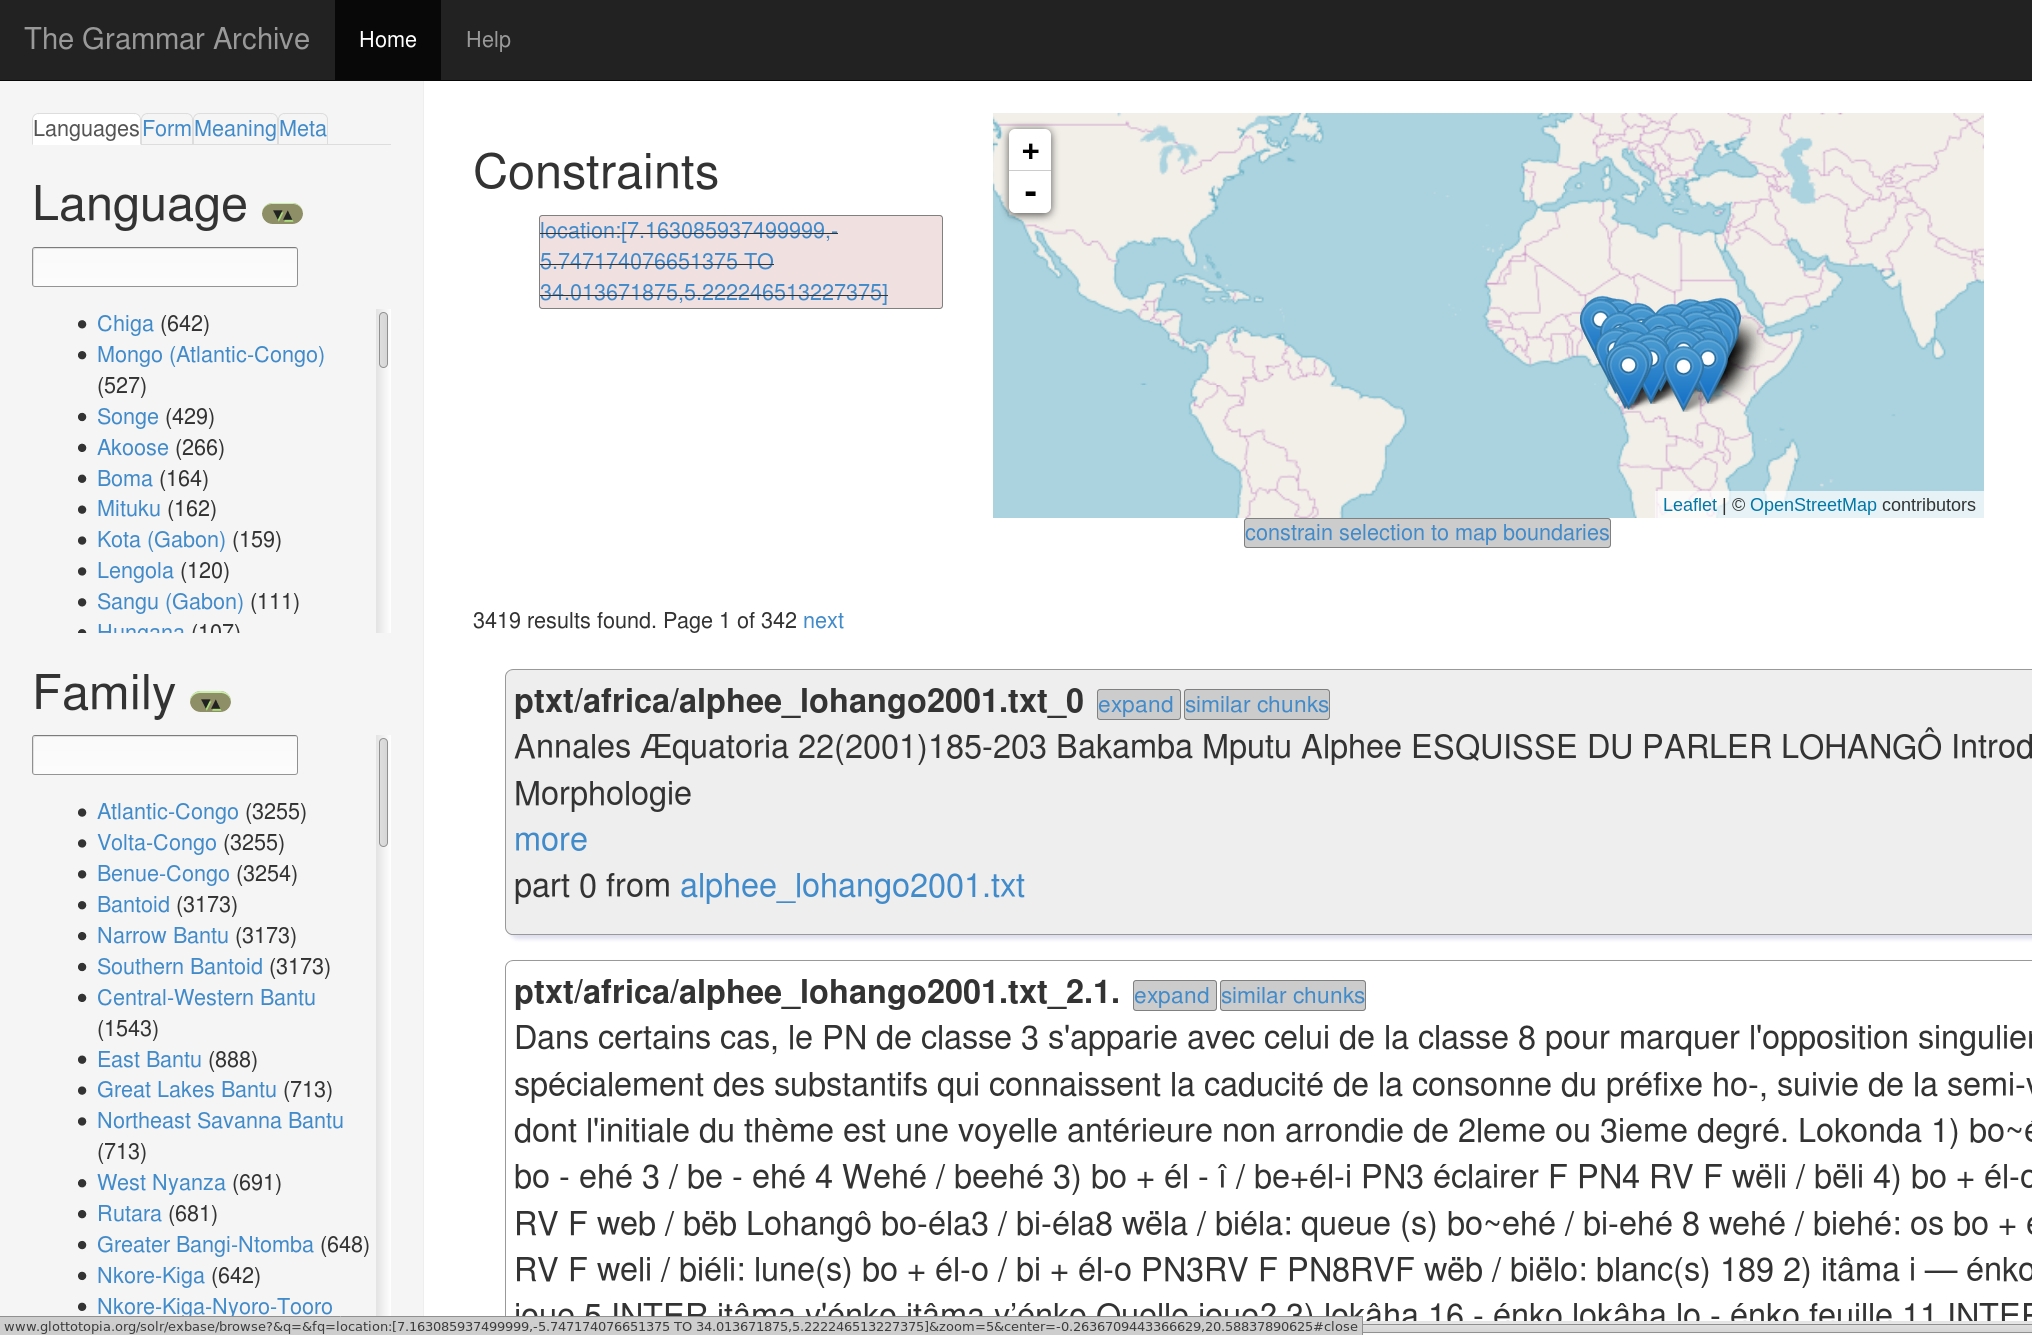
\includegraphics[height=\textheight]{pics/geobox.png} 
}


\frame{
\frametitle{Formal search: gloss}
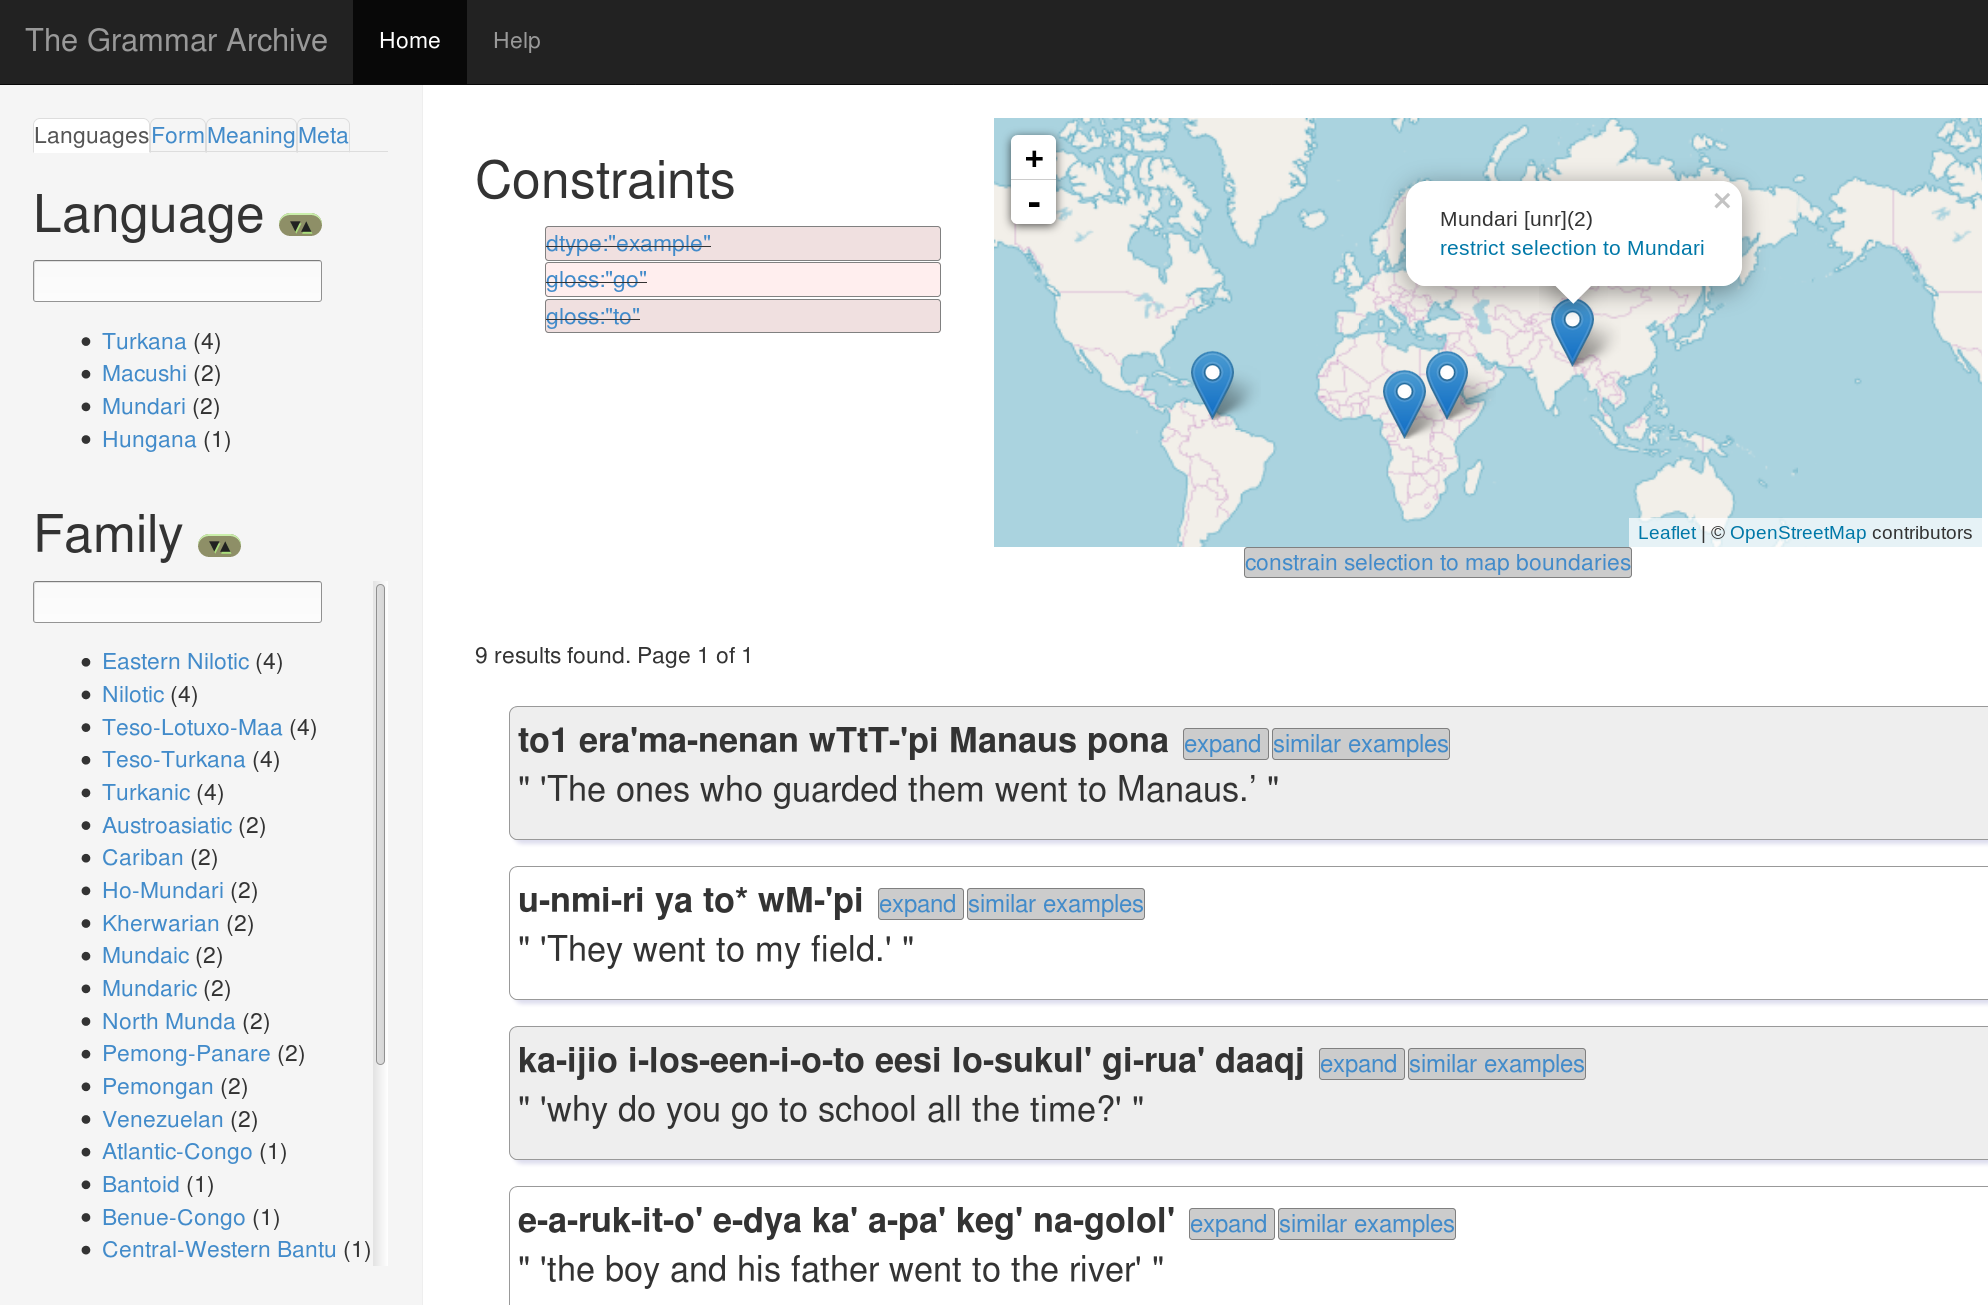
\includegraphics[height=\textheight]{pics/gloss.png} 
}


\frame{
\frametitle{Formal search: complex\newline sentence}
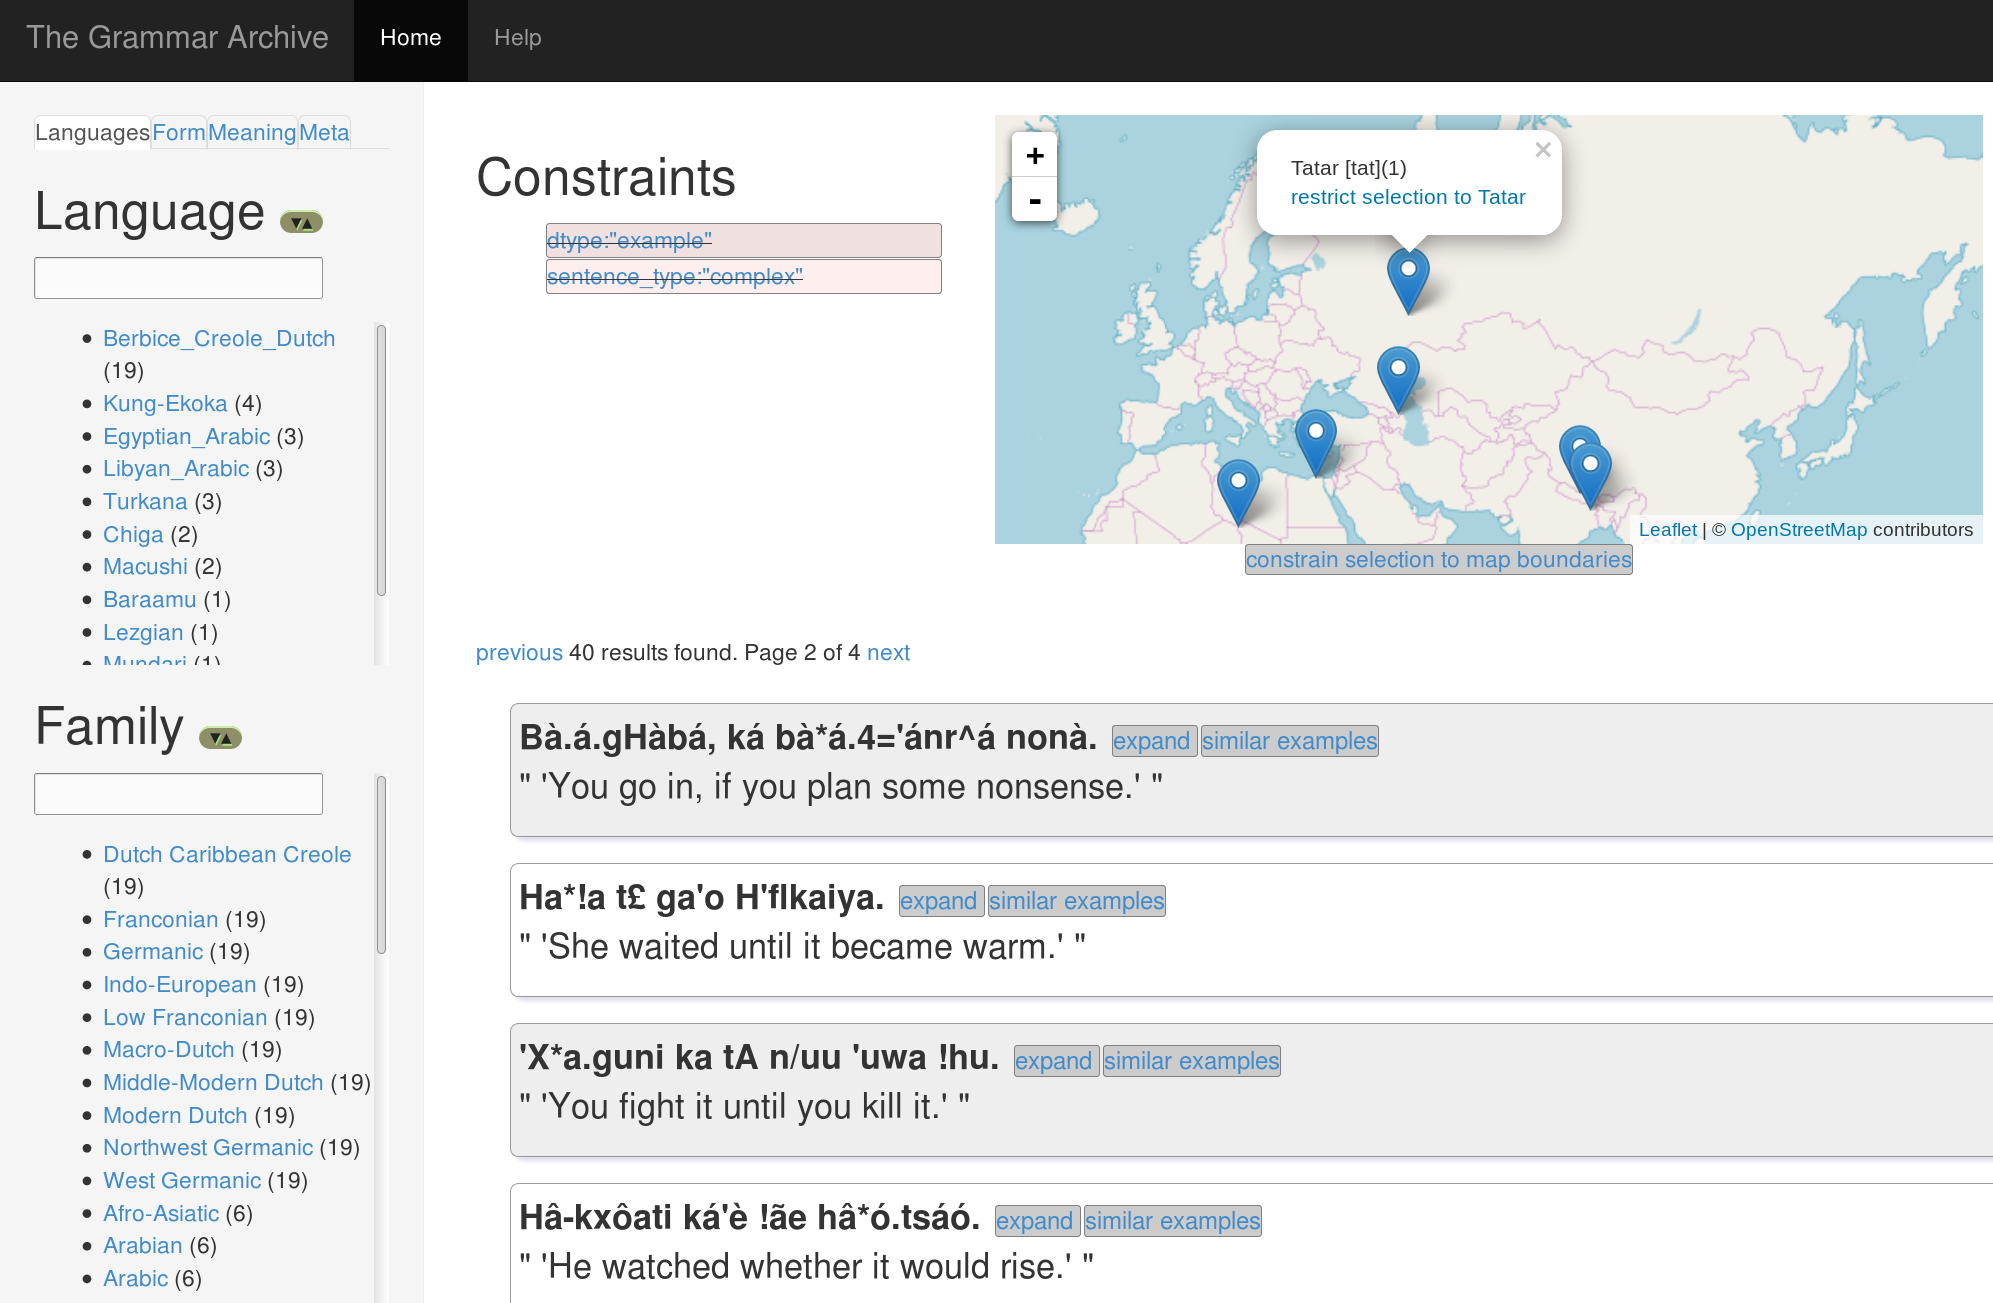
\includegraphics[height=\textheight]{pics/complex.png} 
}


\frame{
\frametitle{Formal search: vernacular\newline  word}
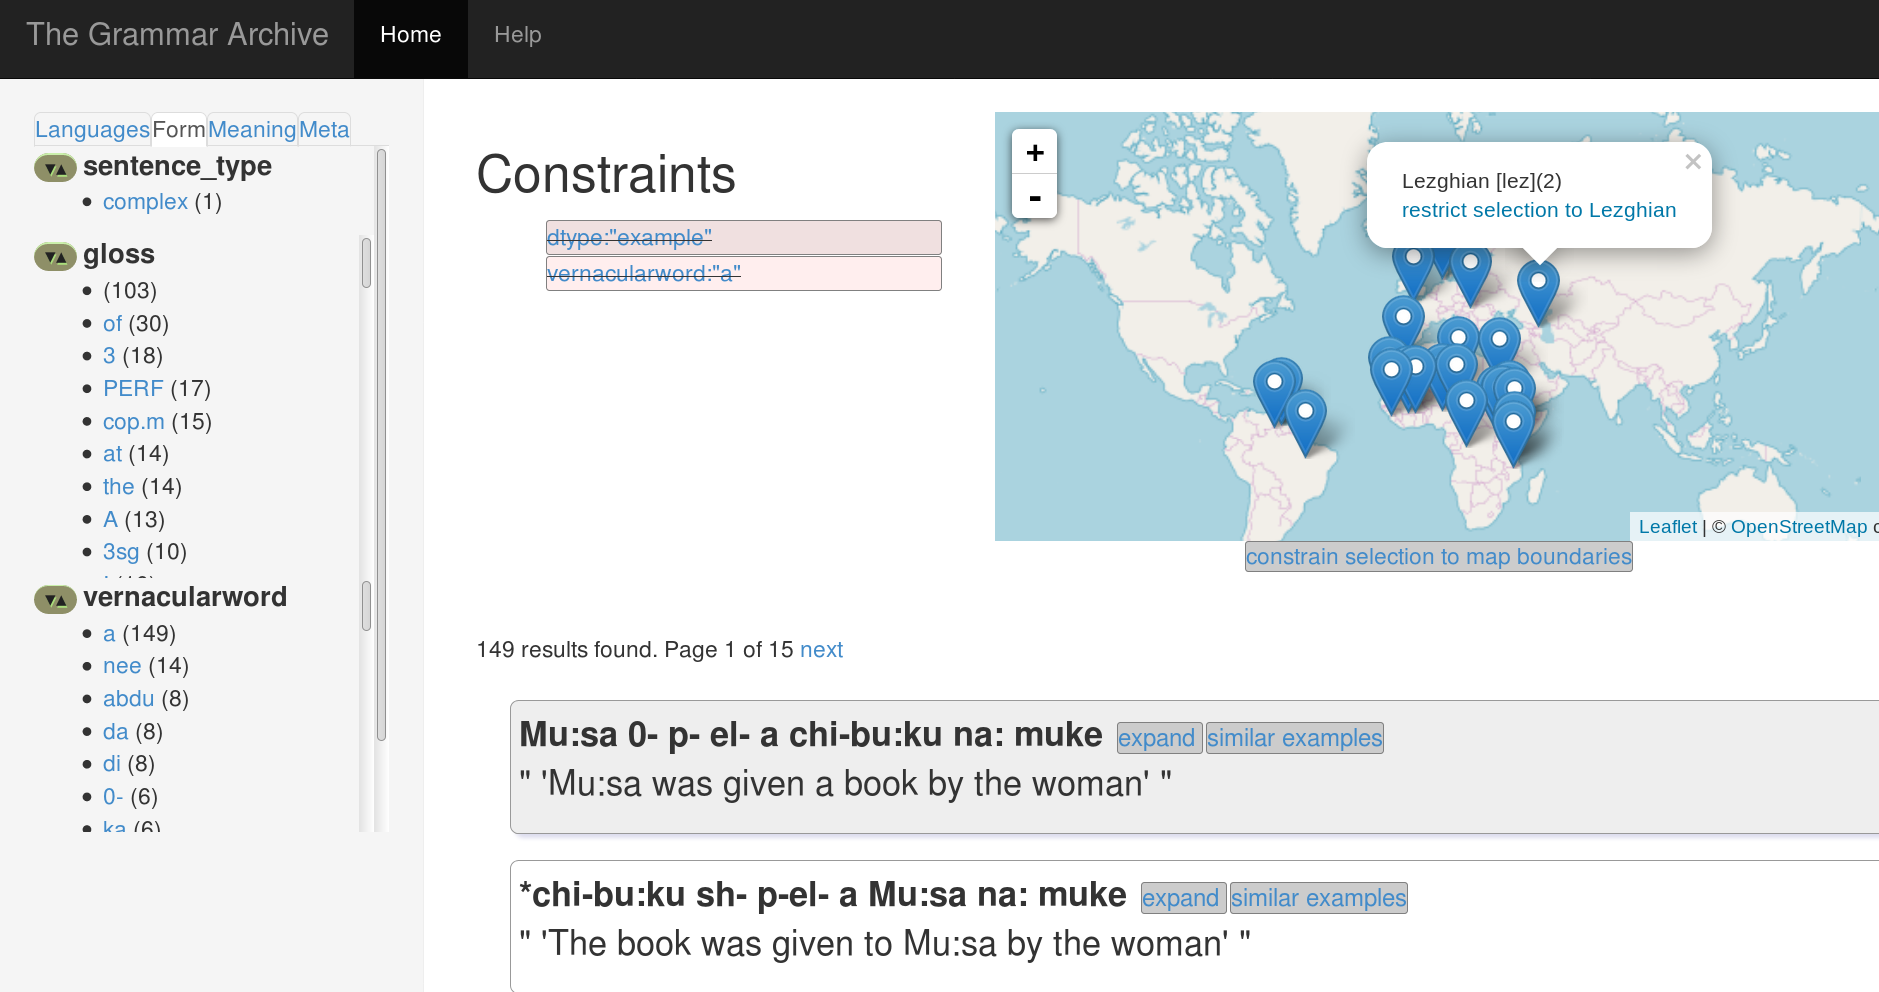
\includegraphics[height=\textheight]{pics/vernacularword.png} 
}
 
% \frame{
% \frametitle{Formal search$^2$: complex sentence + negation}
% 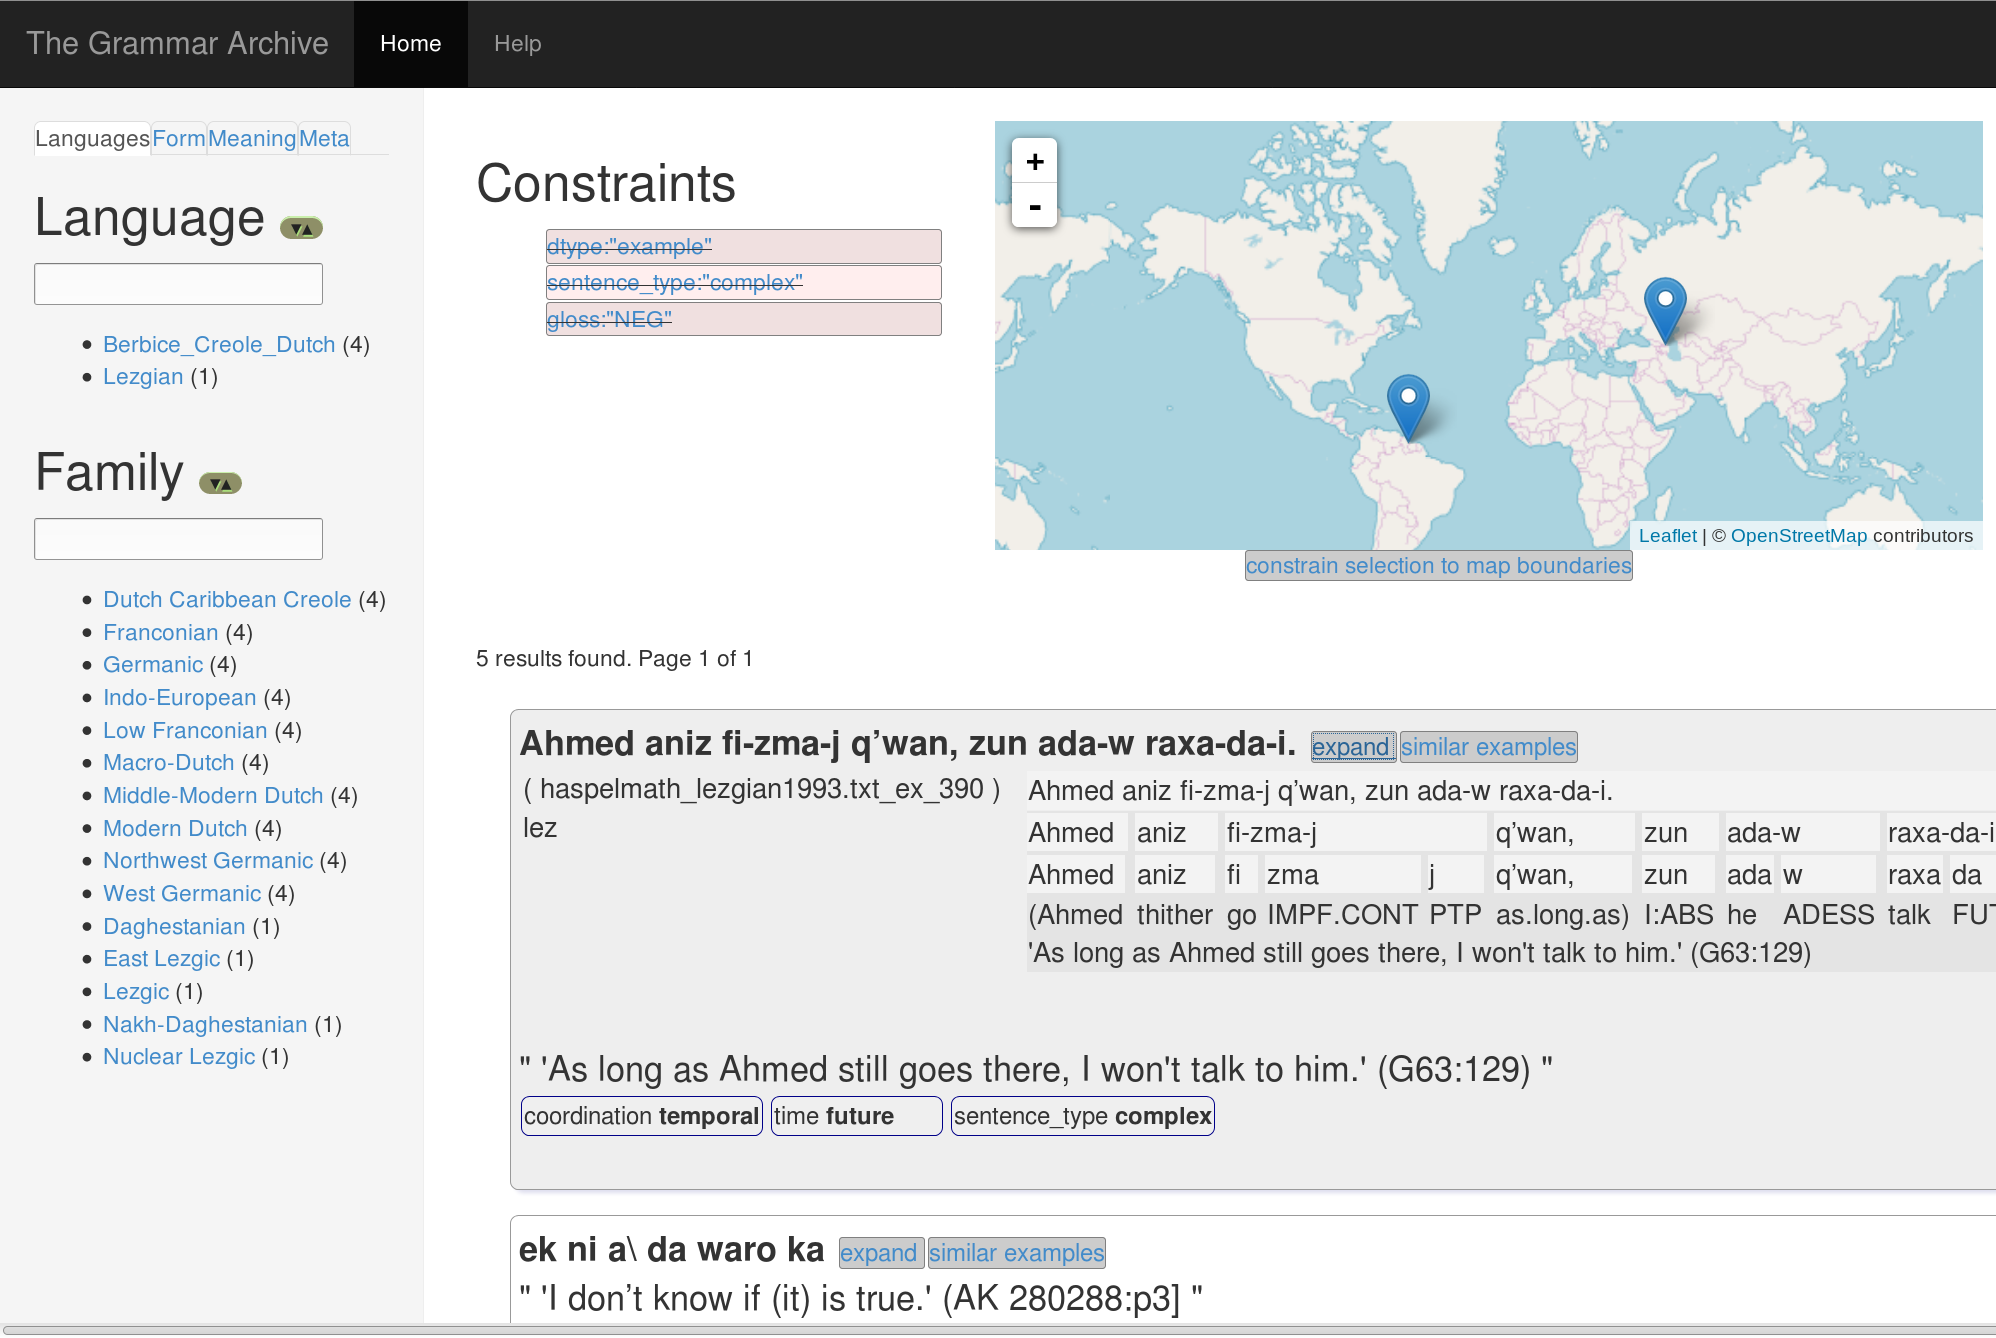
\includegraphics[height=\textheight]{pics/complexneg.png} 
% }
 

\frame{
\frametitle{Meaning search: source}
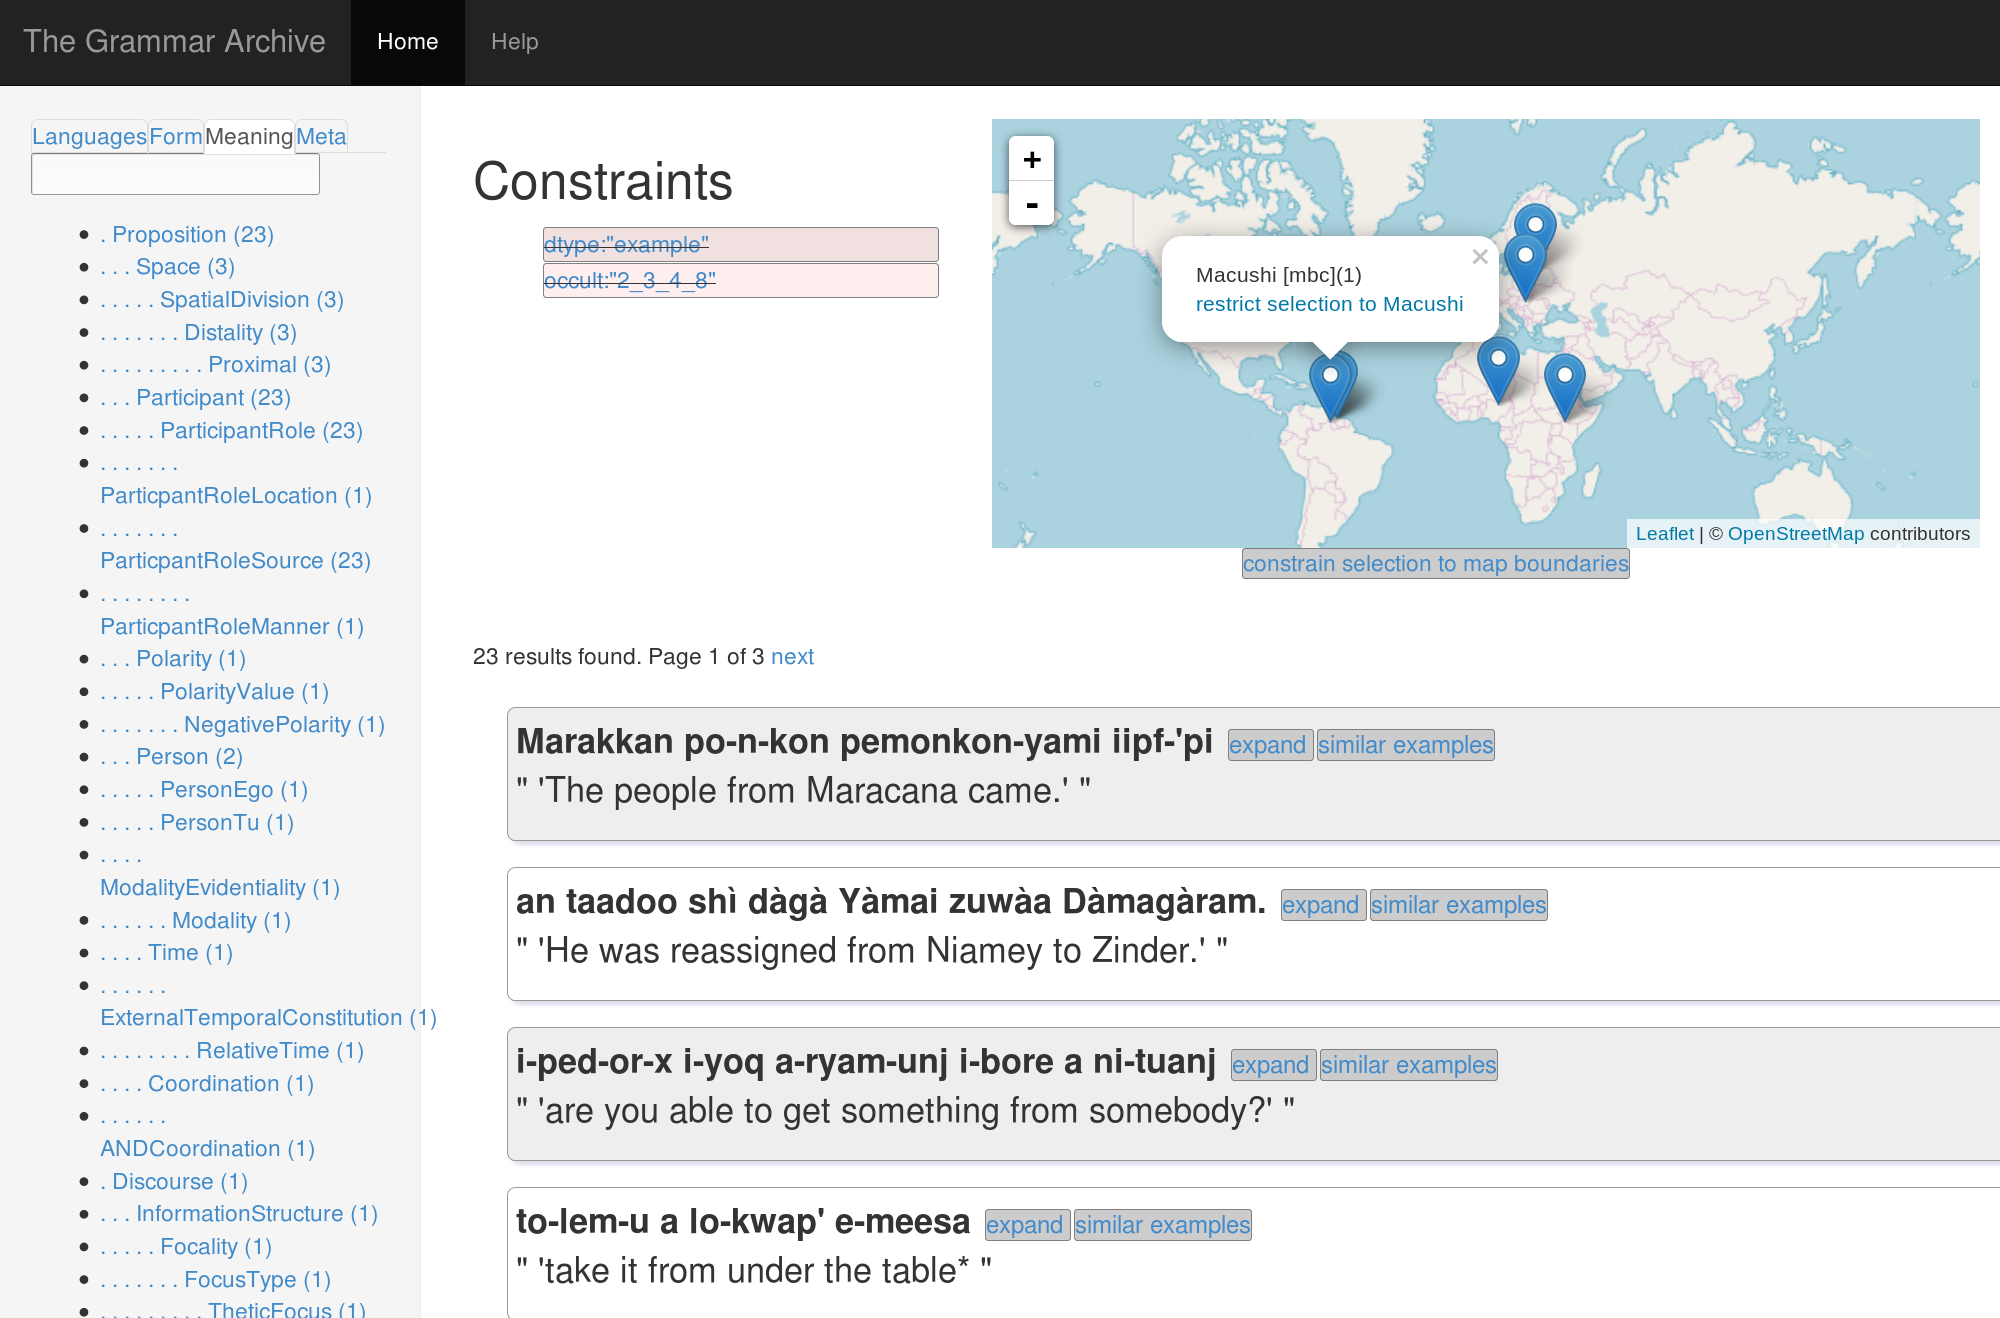
\includegraphics[height=\textheight]{pics/meaningsource.png} 
}
 
\frame{
\frametitle{Complex meaning search: source + proximal}
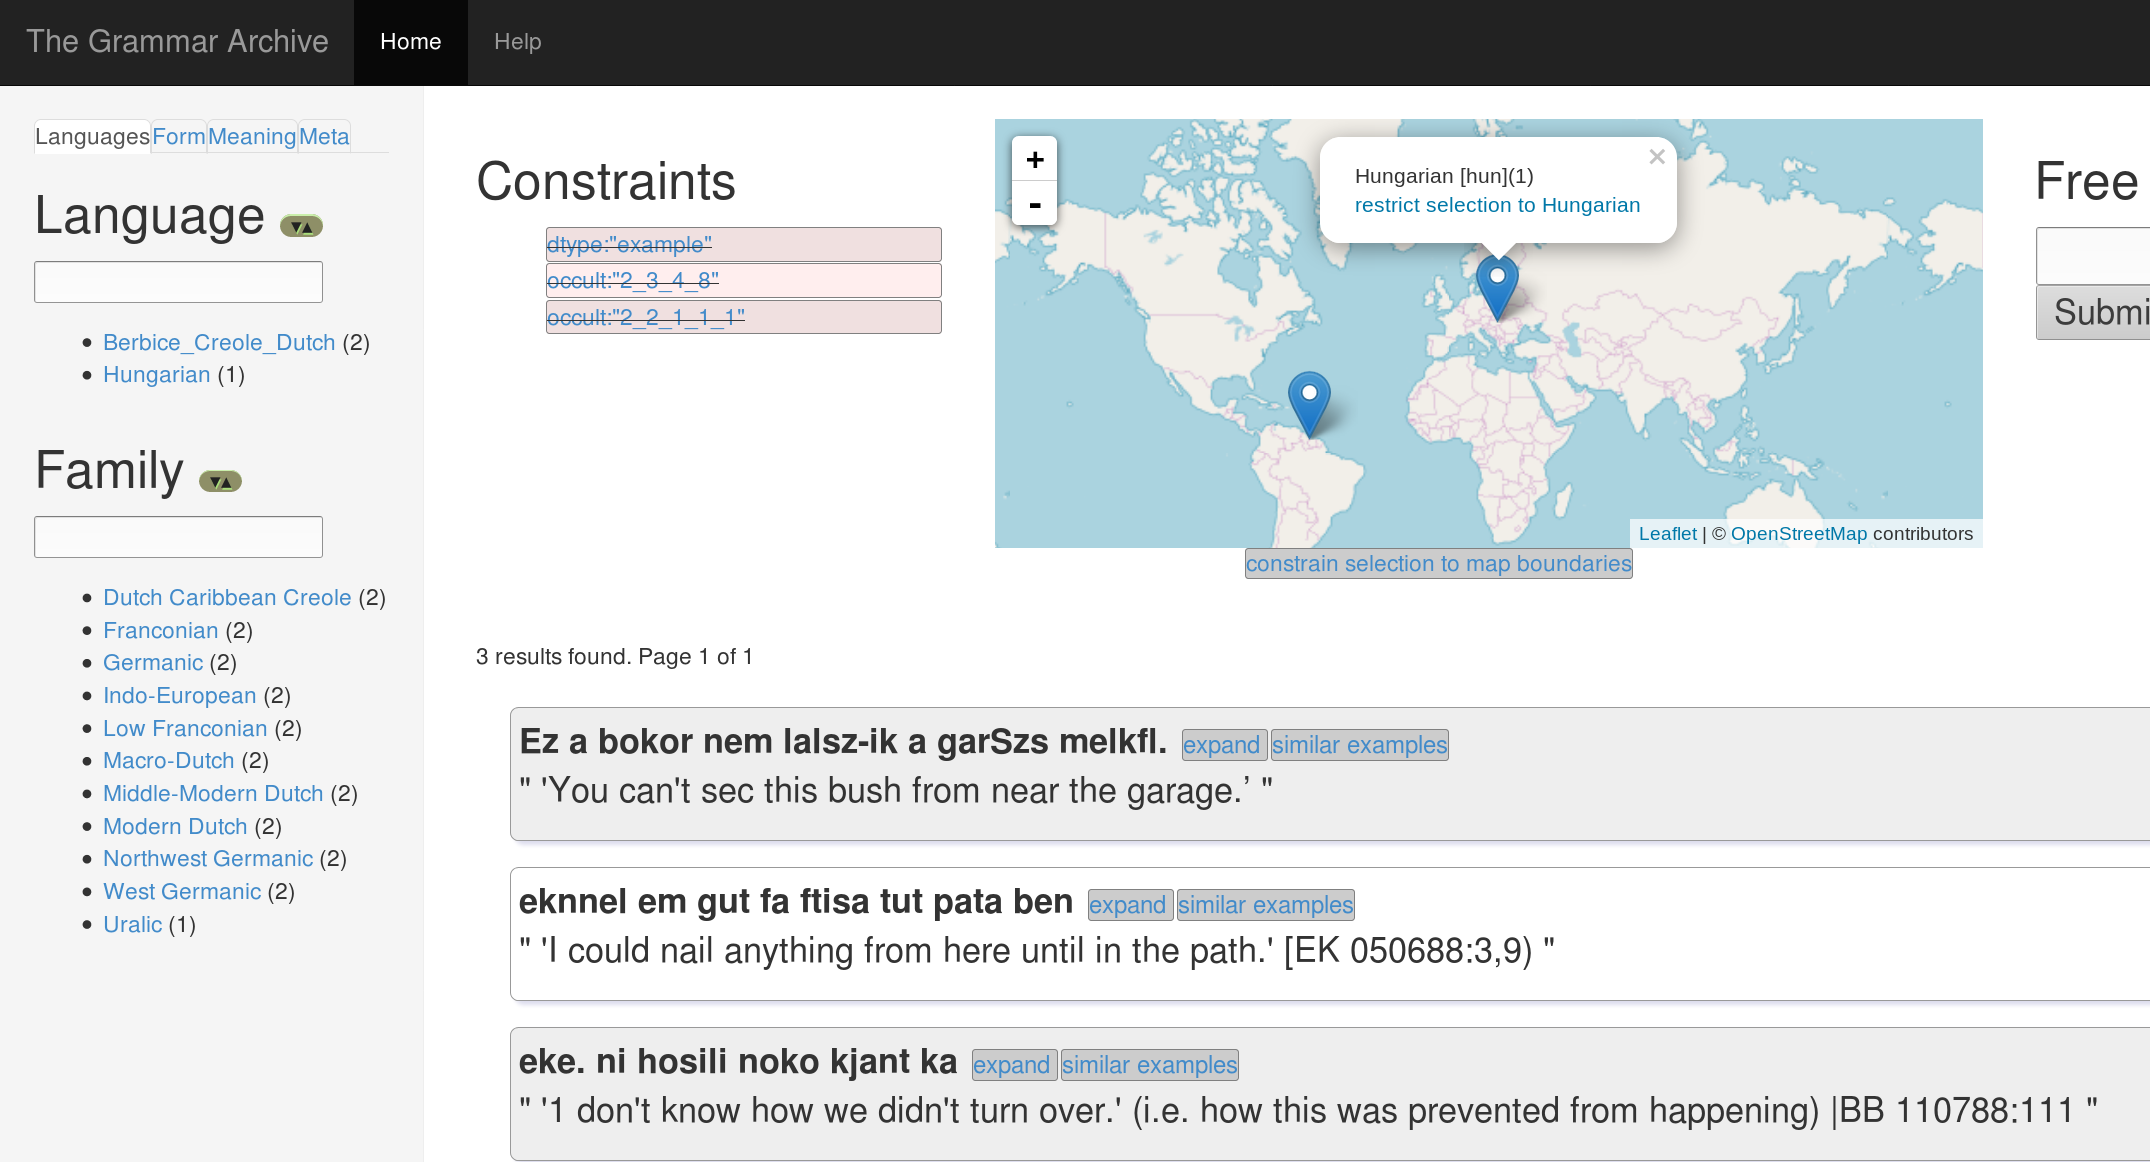
\includegraphics[height=\textheight]{pics/sourceproximal.png} 
}
 
 
\frame{
\frametitle{Similarity search}
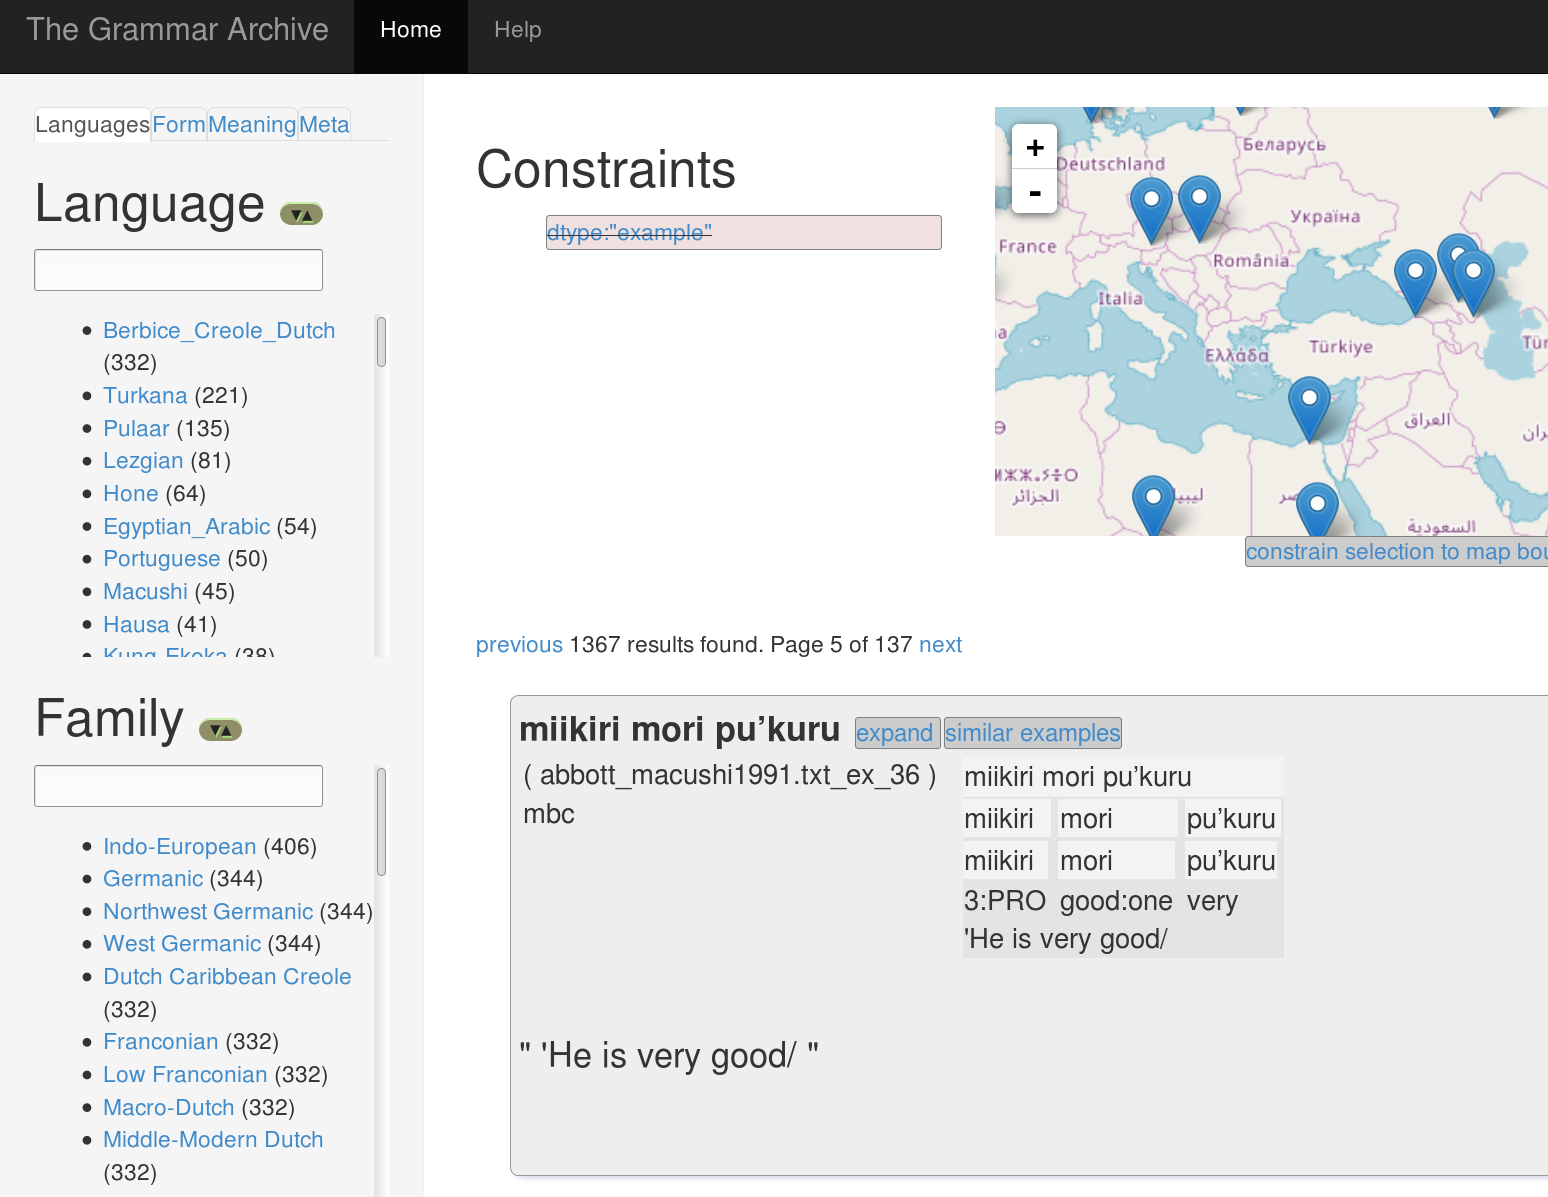
\includegraphics[height=\textheight]{pics/similarI.png} 
}

\frame{
\frametitle{Similarity search}
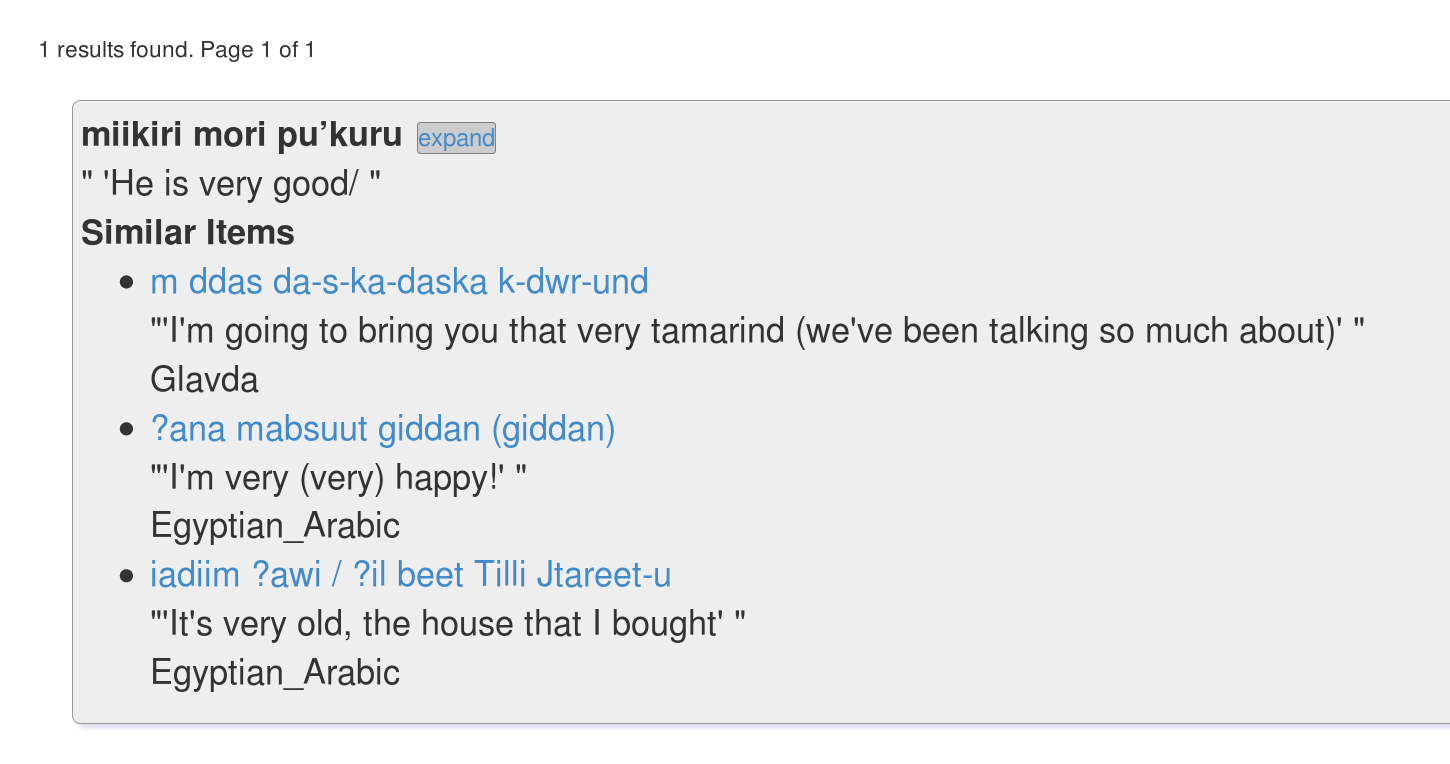
\includegraphics[width=\textwidth]{pics/similarII.png} 
}


\frame{
\frametitle{Free search}
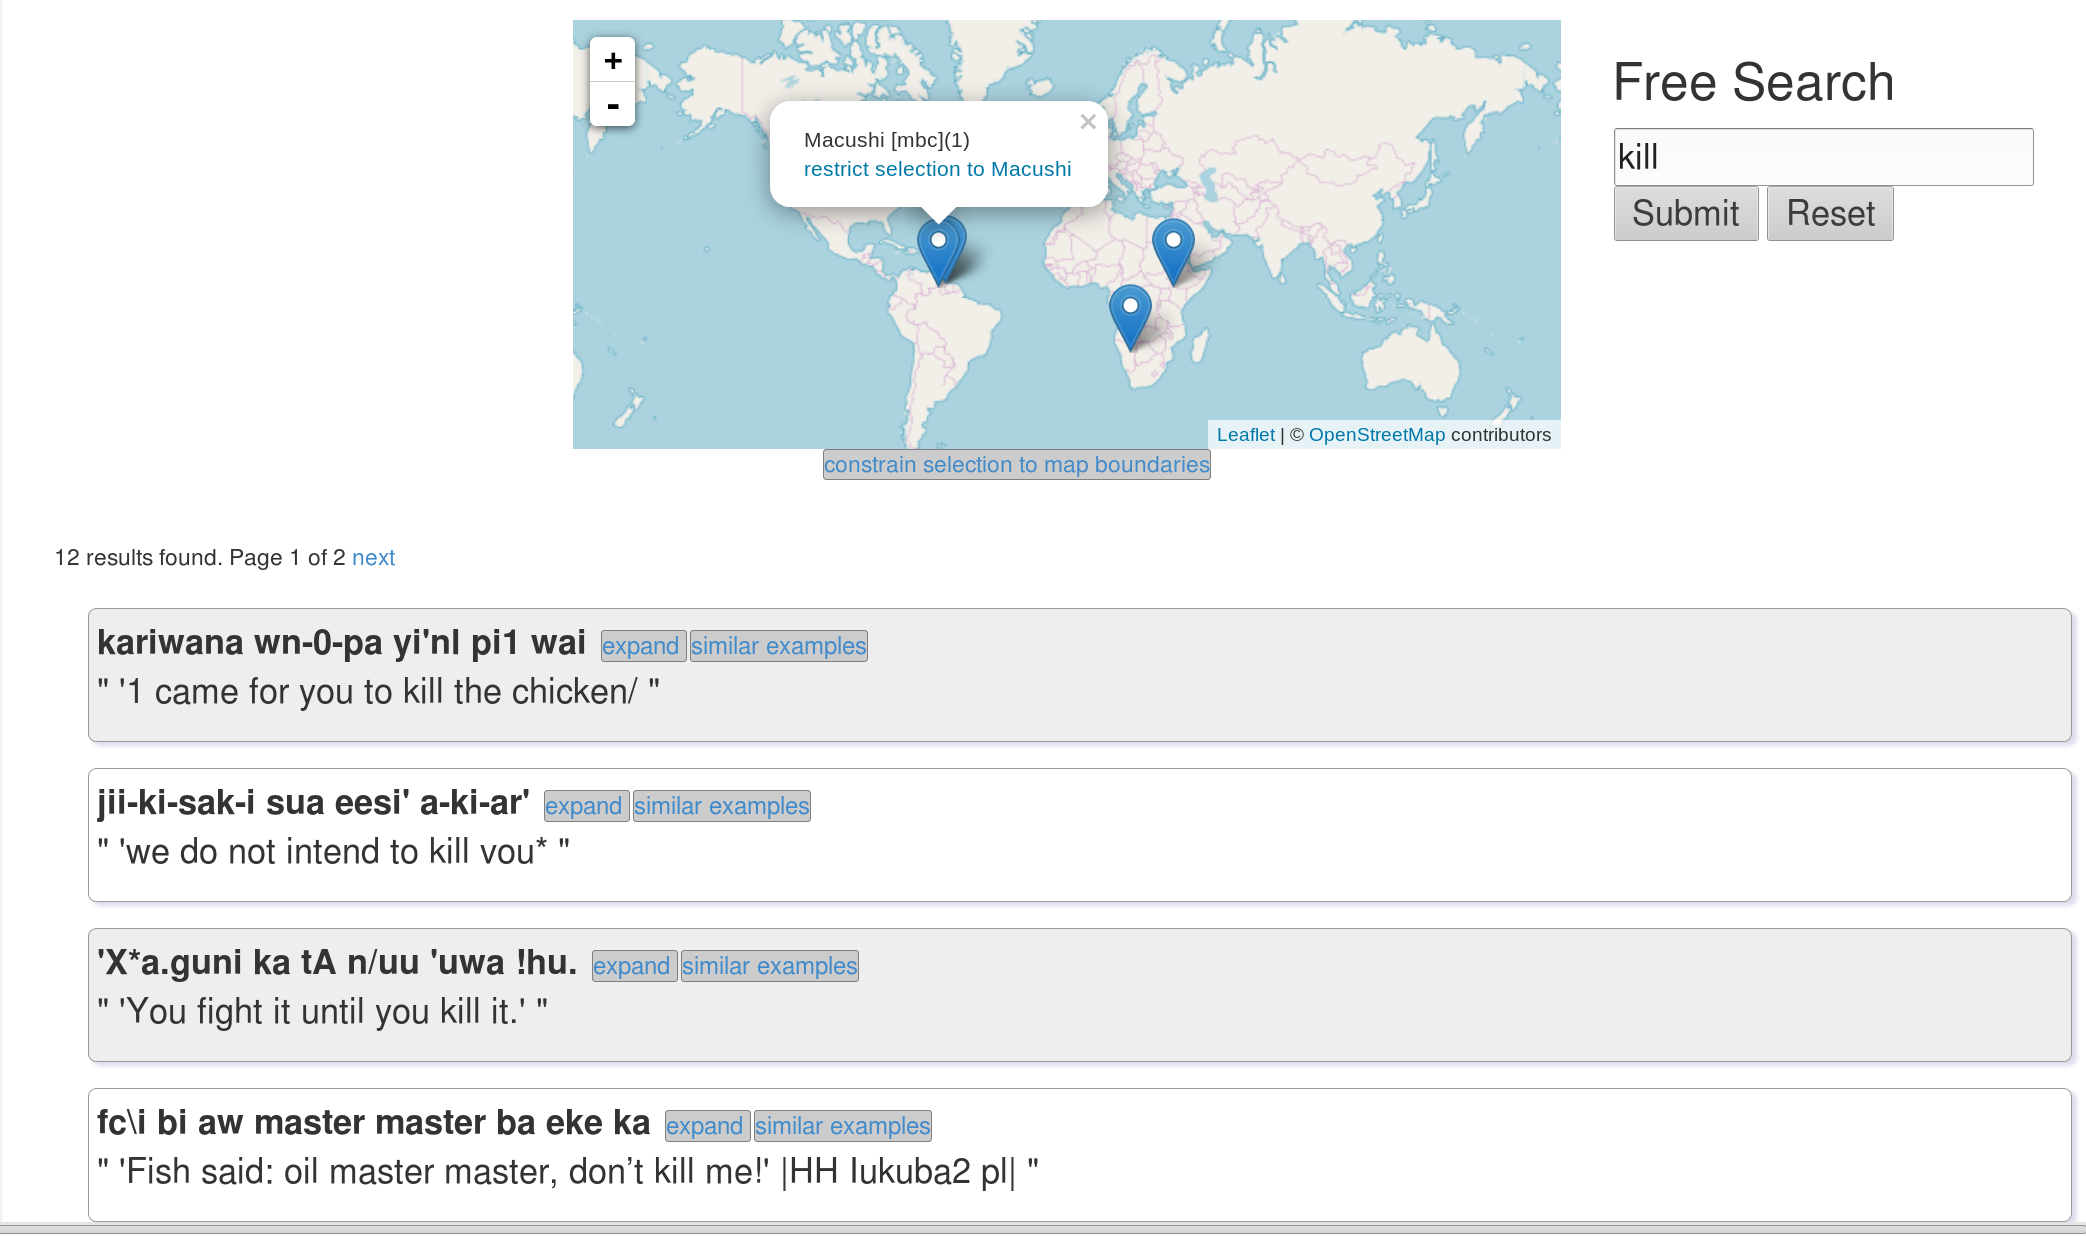
\includegraphics[width=\textwidth]{pics/freesearch.png} 
}



\frame{
\frametitle{Free search}
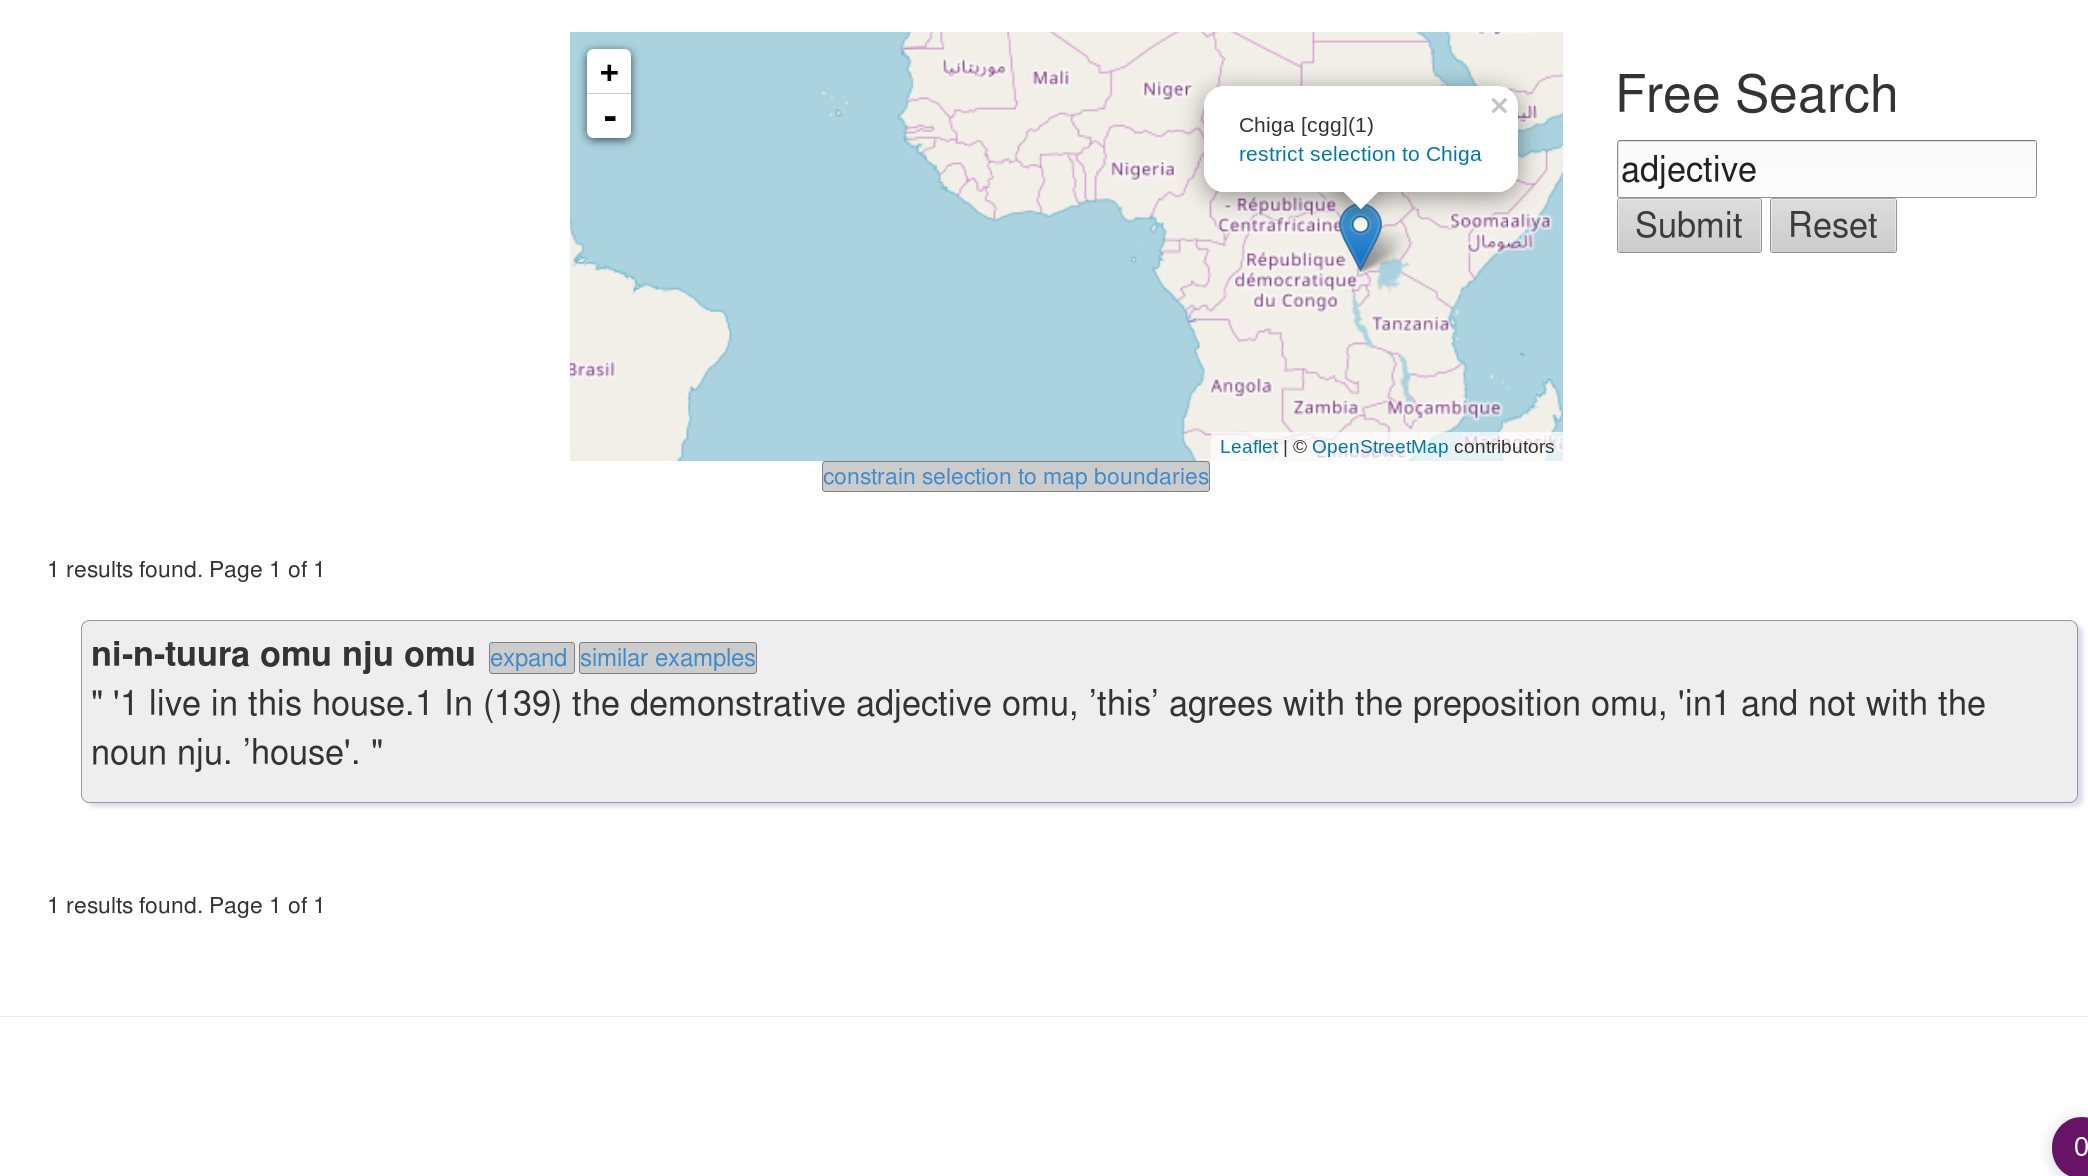
\includegraphics[height=\textheight]{pics/adjective1.png} 
}


\frame{
\frametitle{Free search: text}
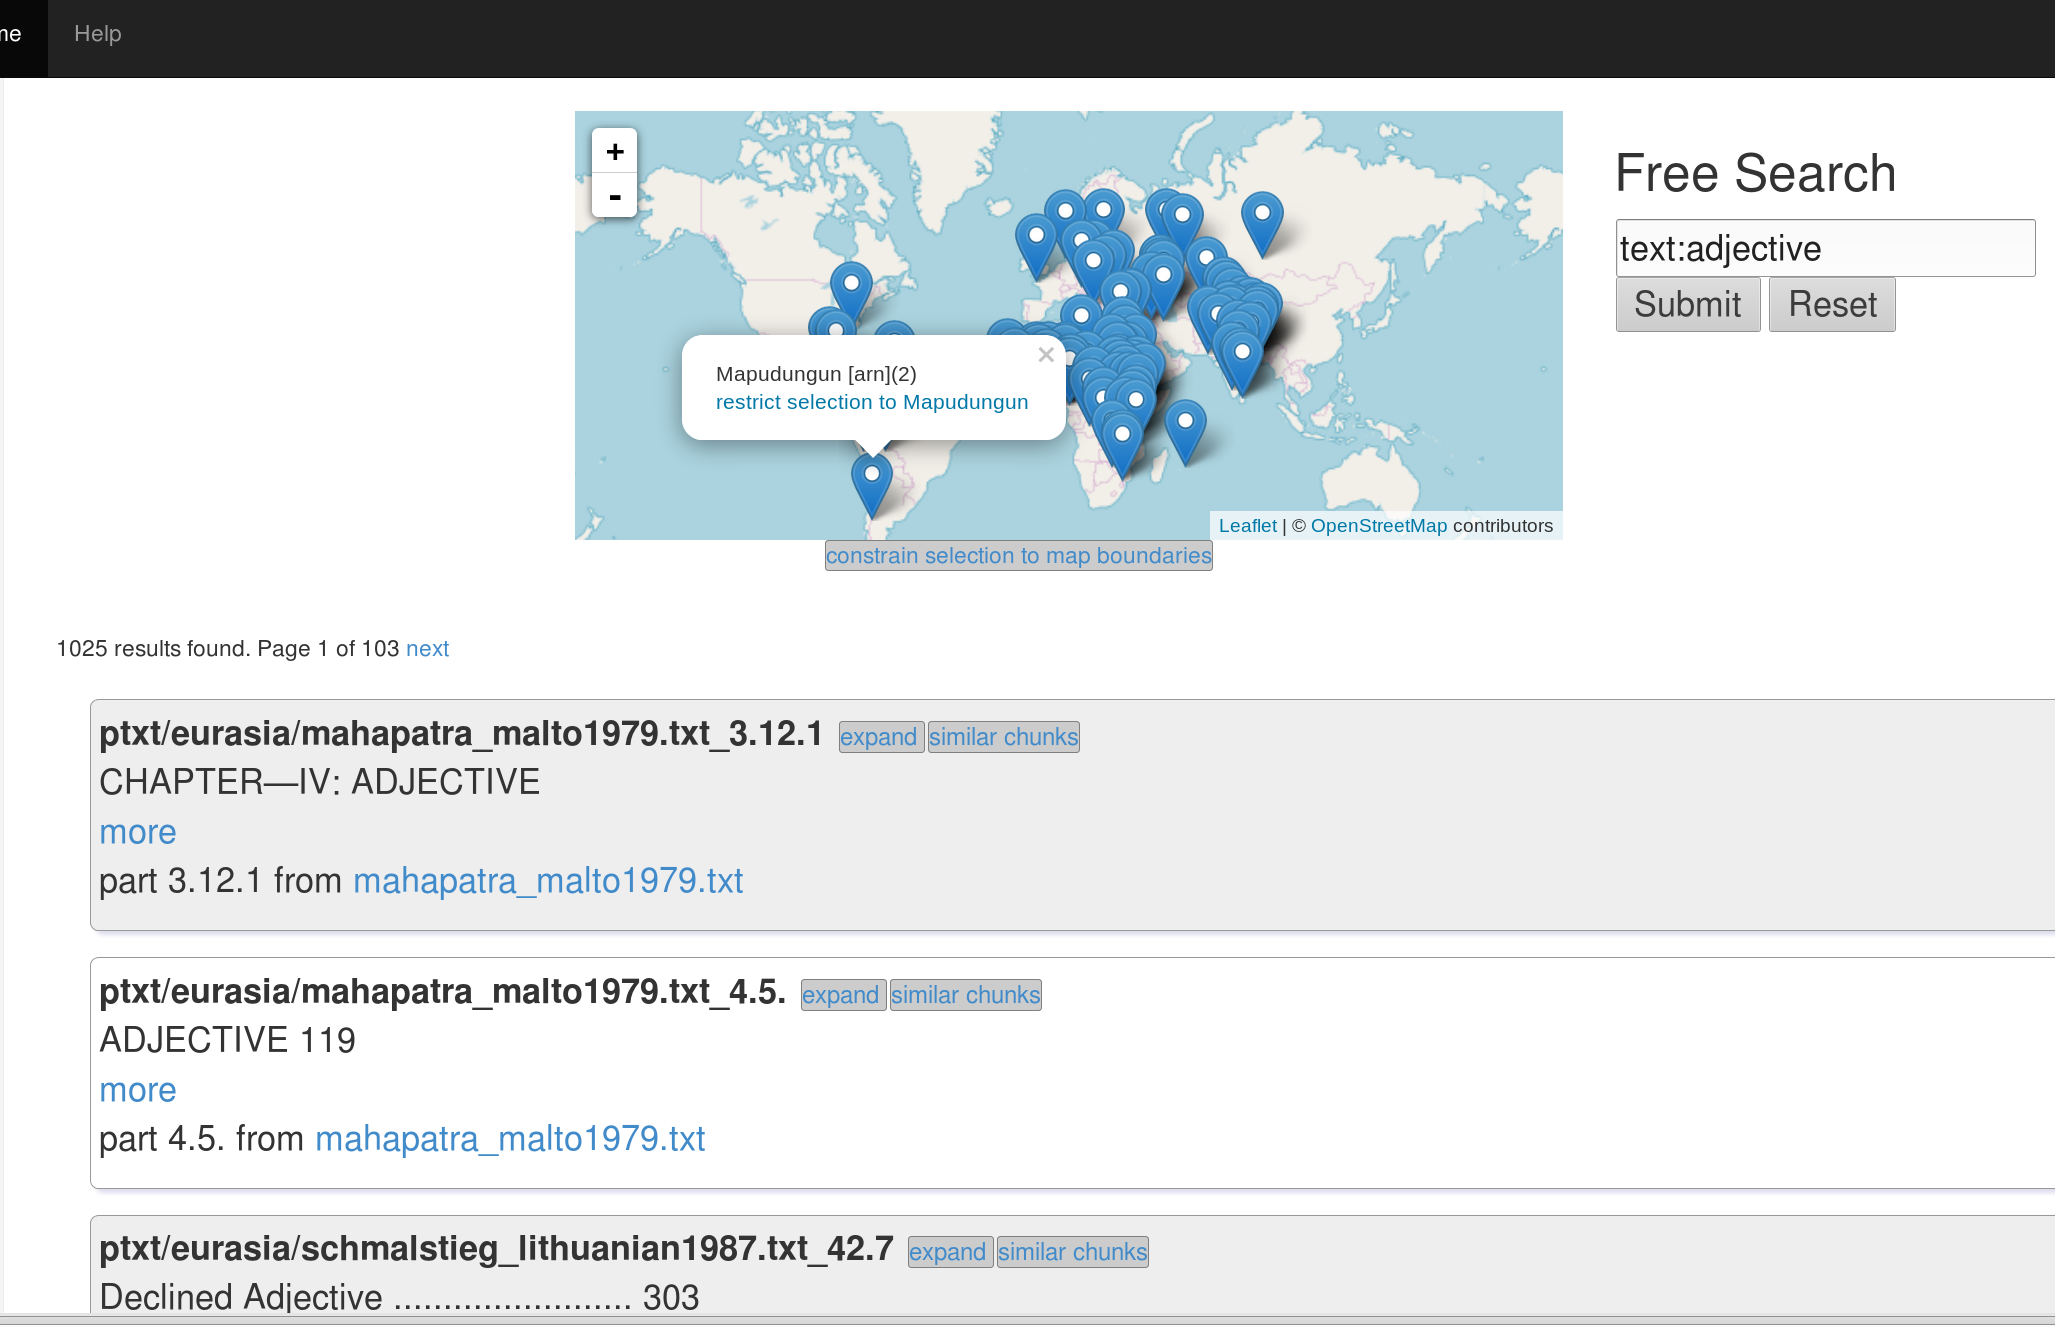
\includegraphics[height=\textheight]{pics/adjective2.png} 
}


\frame{
\frametitle{Free search: text (fuzzy)}
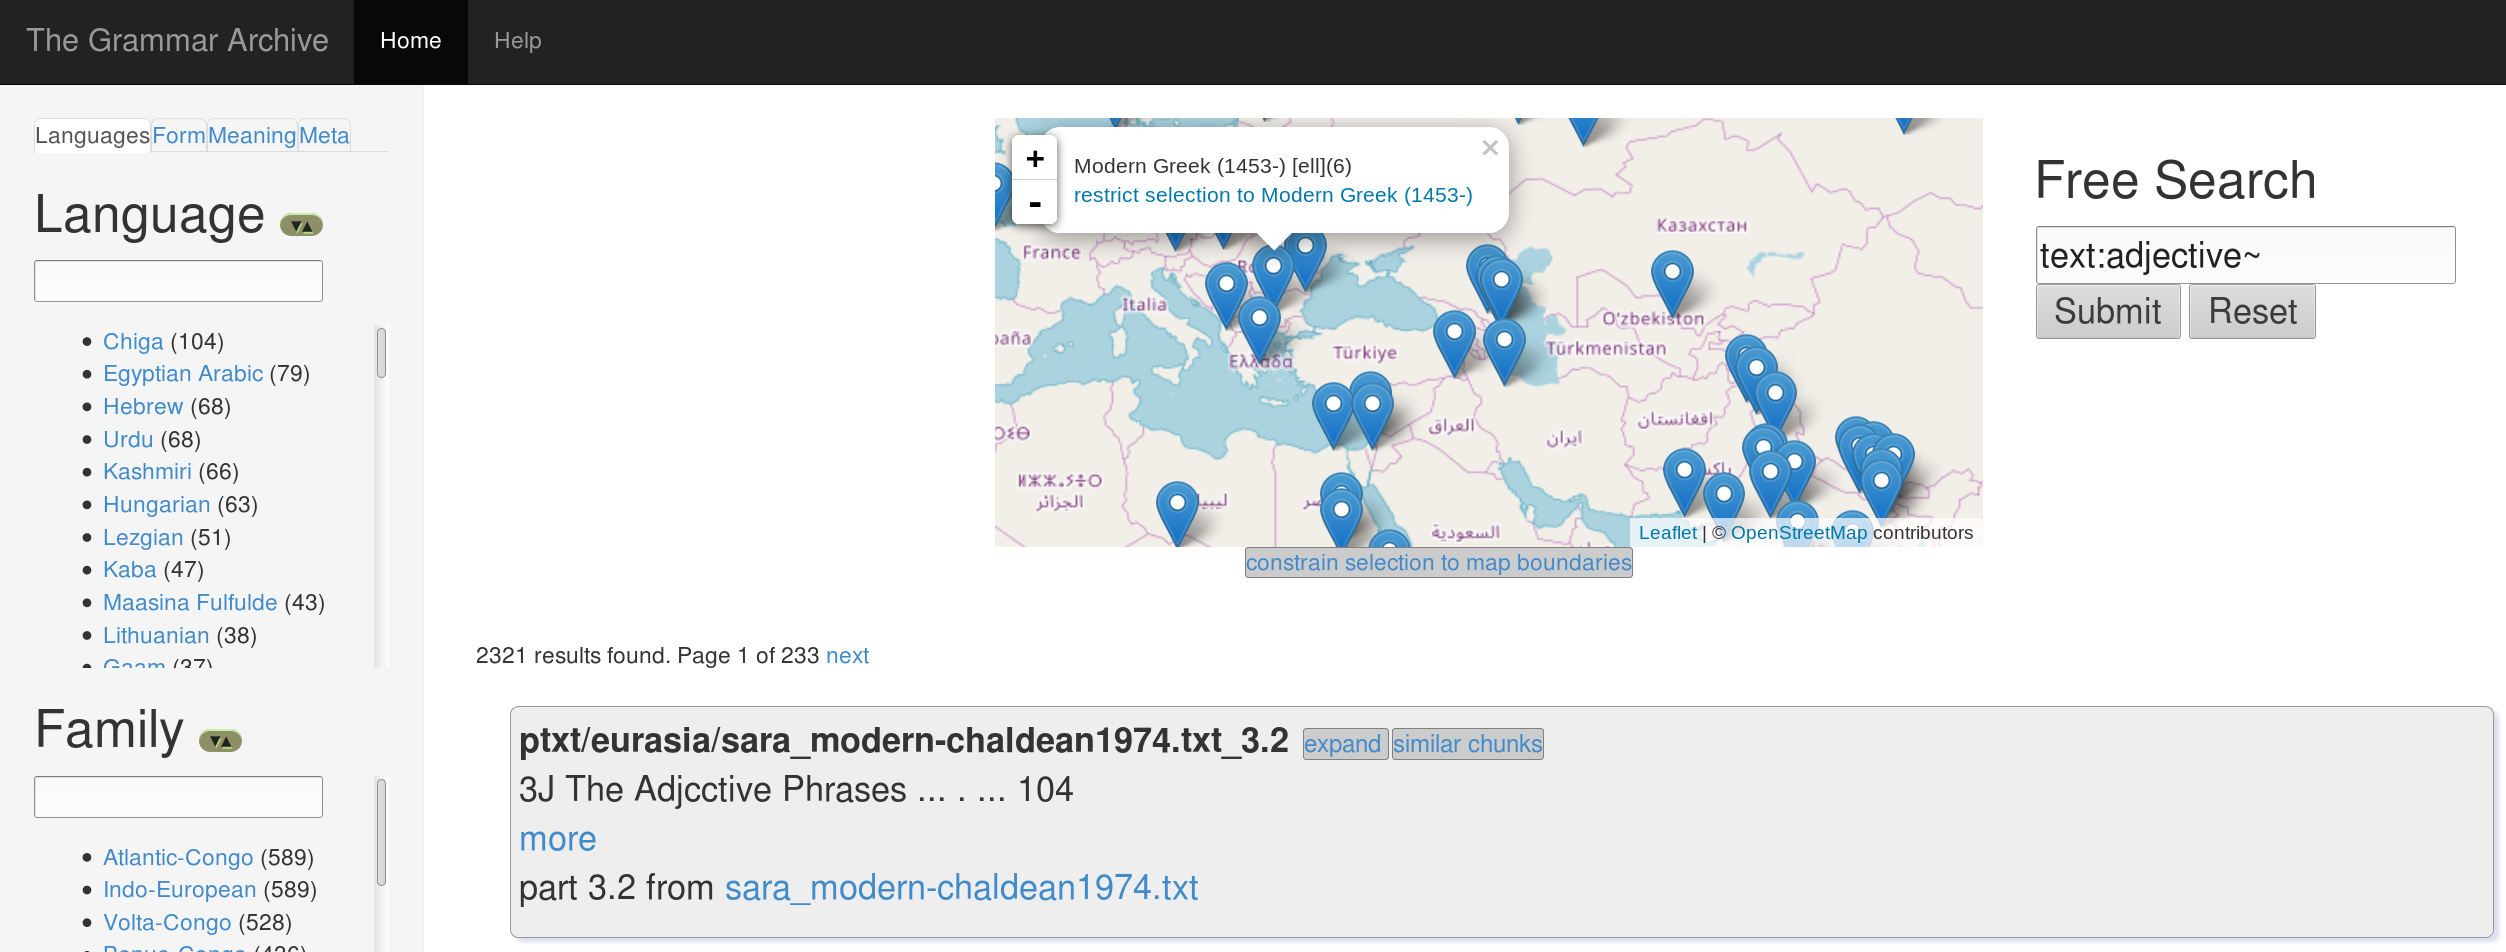
\includegraphics[width=\textwidth]{pics/adjective3.png} 
}


% \frame{
% \frametitle{Free search: geographical\newline distribution of the paucal}
% 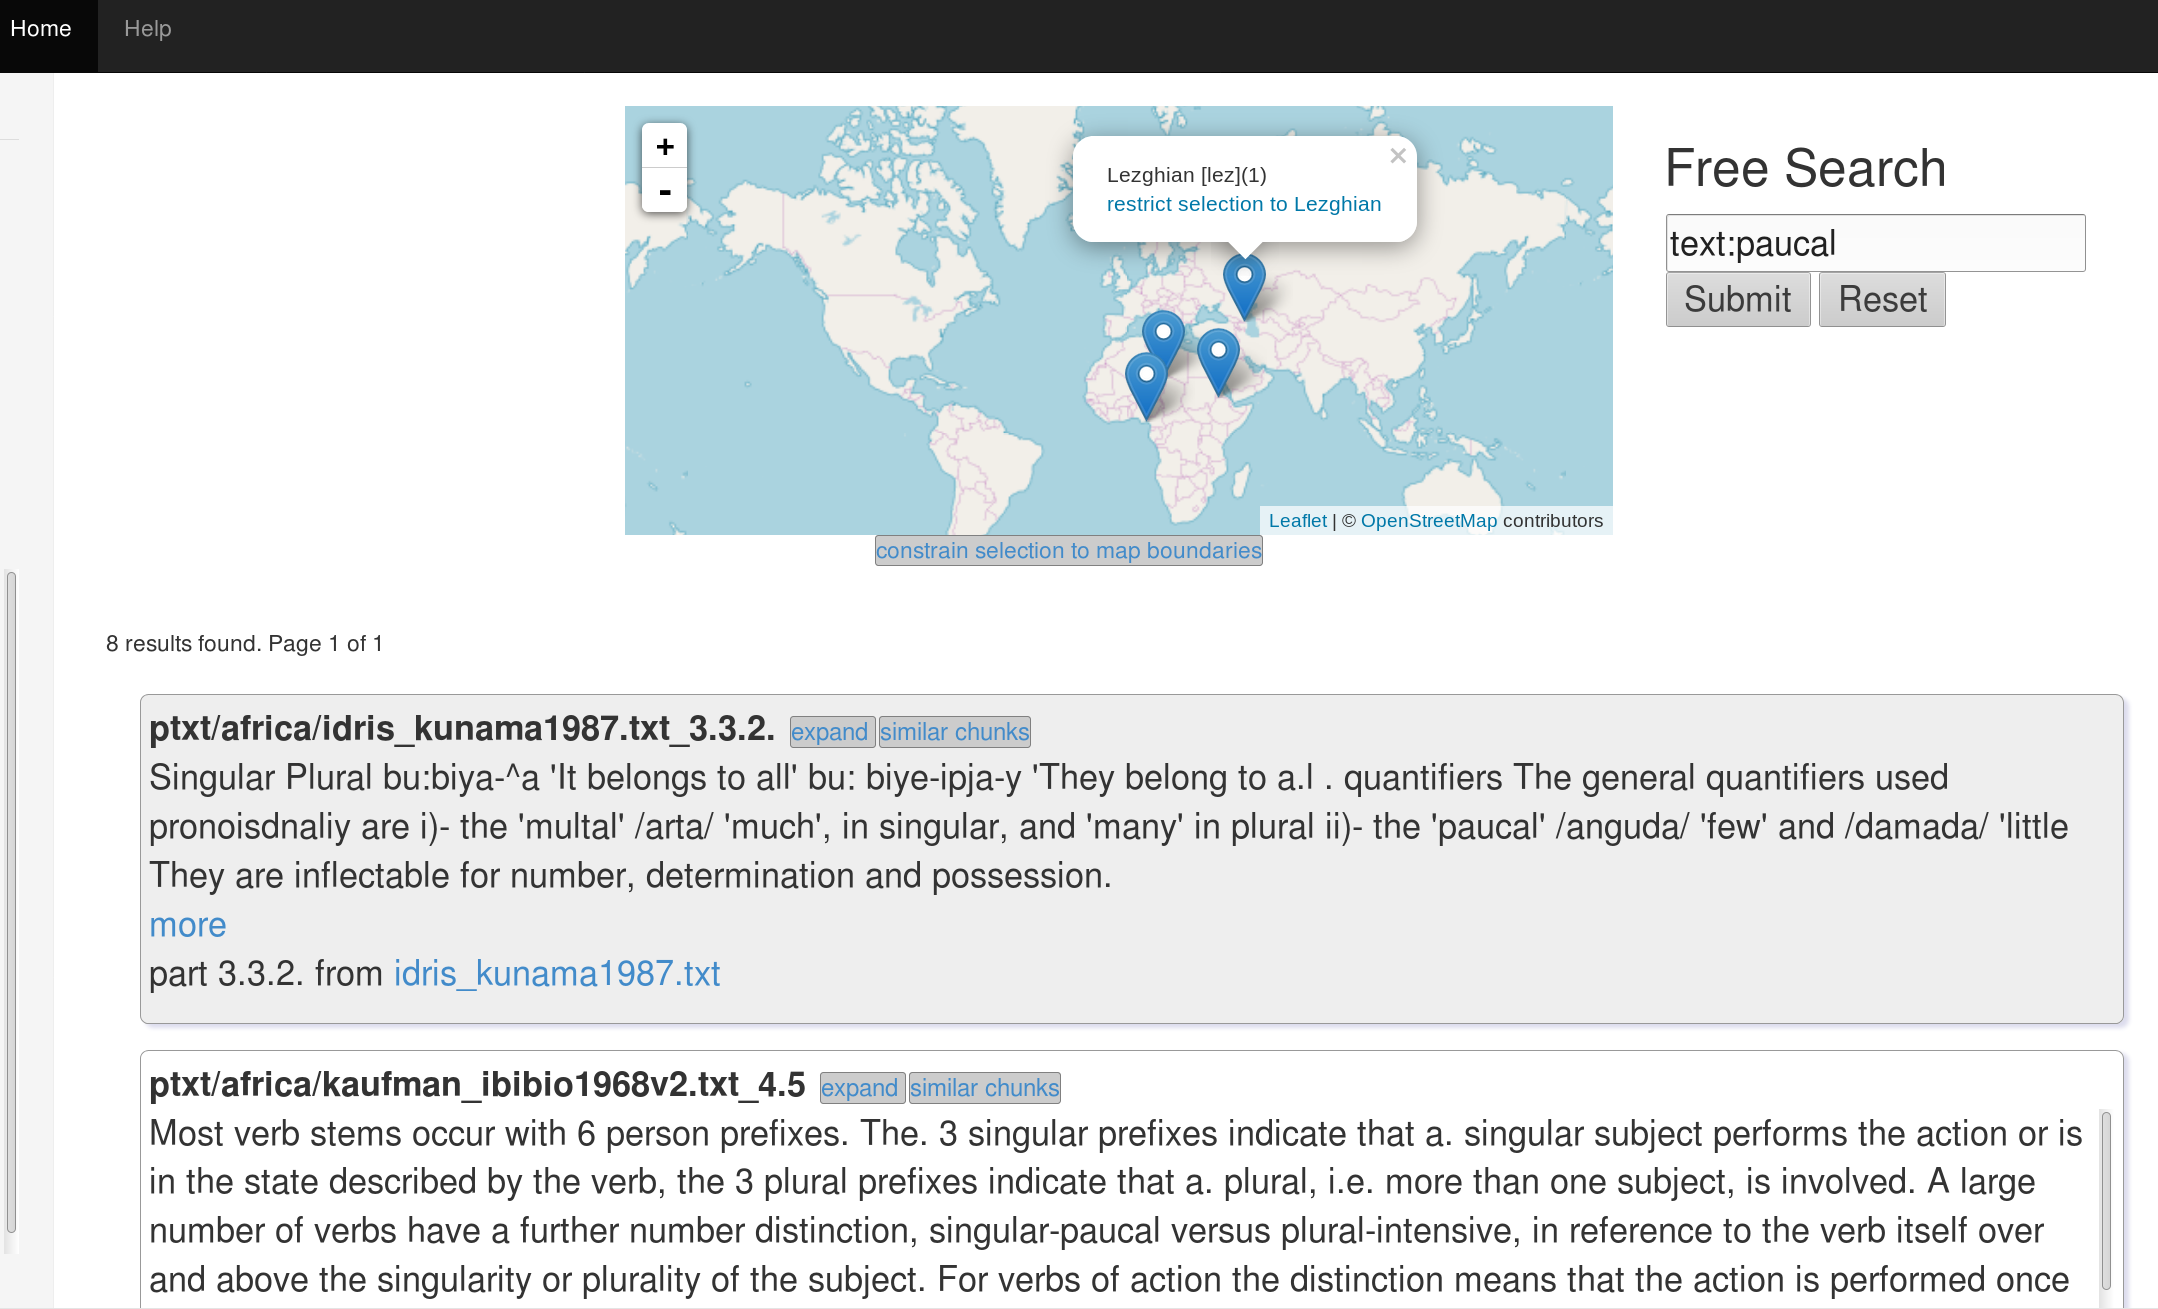
\includegraphics[height=\textheight]{pics/paucal.png} 
% }


\frame{
\frametitle{Complex search: form + meaning + geneaology + geo}
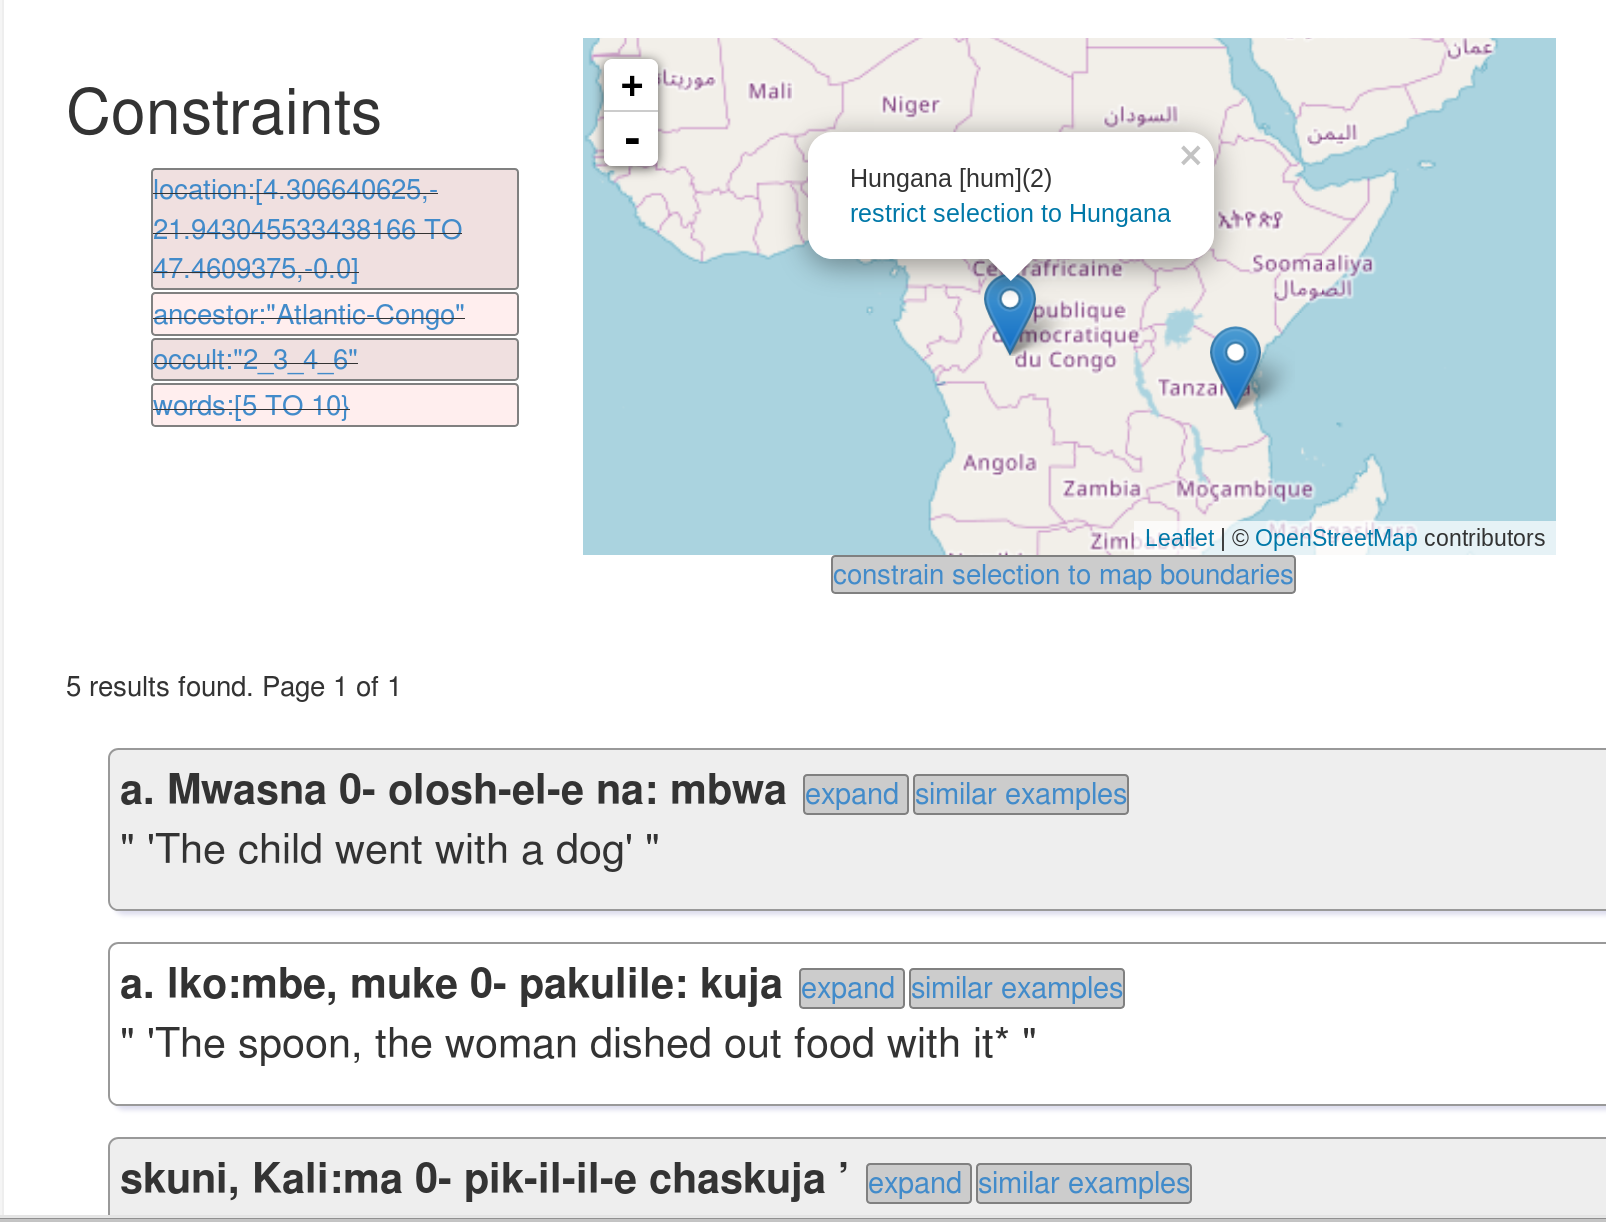
\includegraphics[height=\textheight]{pics/combination.png} 
}

\frame{
\frametitle{Machine-readable version}
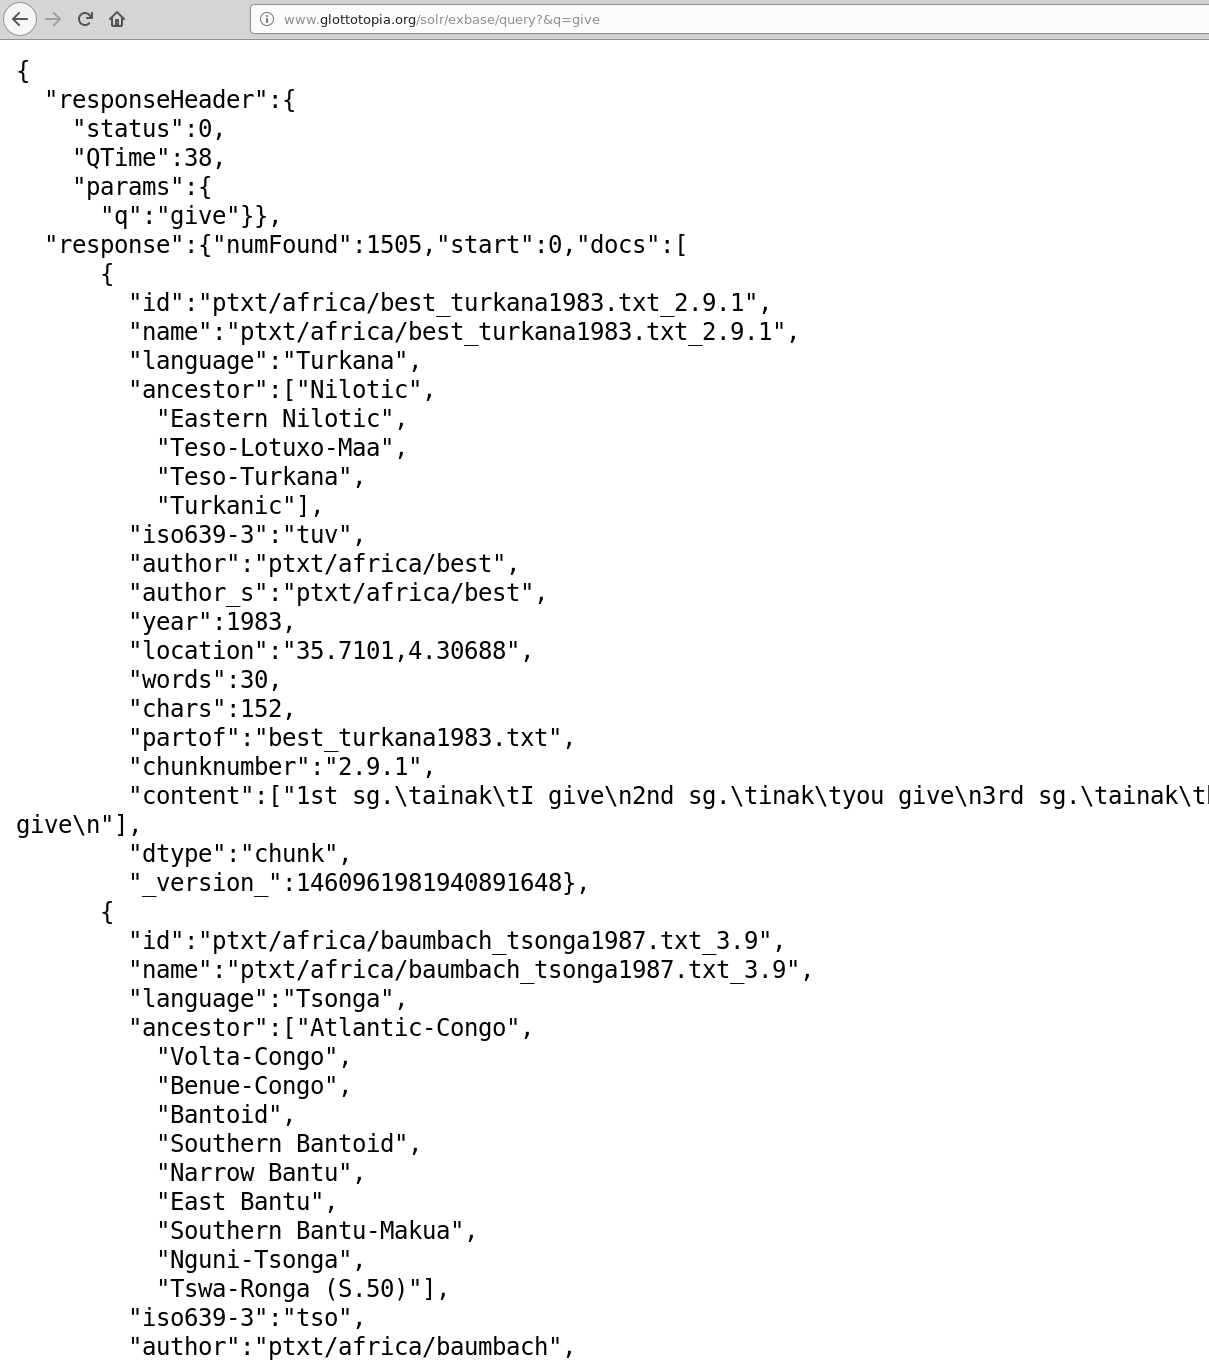
\includegraphics[height=\textheight]{pics/json.png} 
} 




\section{Expansion}
\frame{
\frametitle{Expansion}
%   \includegraphics[height=.2\textheight]{./path/to/graphicsfile}
  \begin{itemize}
    \item  currently only 1300 ``vanilla'' examples from HH's grammars
    \item APiCS has 15k examples 
    \item LangSci books have another 15k examples
    \item Open Text Collections (DFG grant proposal pending) has another 80k examples 
  \end{itemize}
}


\section{Technical background}
\frame{
\frametitle{Technical background}
\begin{itemize}
\item Apache SOLR search platform
\item  velocity templating engine
\item  Bootstrap layout
\item  jquery user interface
\item  leaflet maps
\item  python import script
\item  Ontology of Comparative Concepts used in Linguistic Typology (OCCULT, Hengeveld \& Nordhoff, draft)
\item  categorisation based on translation
\end{itemize}
}

\section{Conceptual issues}
\frame{
\frametitle{Conceptual issues}
\begin{itemize}
 \item examples are ``bags of words'' and have no internal structure
 \begin{itemize}
  \item \textit{Mais \textbf{vous} disiez qu'il \textbf{s}'était caché} will be retrieved for a query 2\textsc{pl} + \textsc{refl} even if it is not pertinent
 \end{itemize}

 \item naïve approach to cross-linguistic categories
 \begin{itemize}
  \item when author calls something ``ergative'', it will be seen as ergative, period.
  \item readers still have to interpret the result set 
  \item not suitable for (quantitative) analysis, but only for exploration 
 \end{itemize}
 \item underlying ontology probably too complex 
 
\end{itemize}
}

\frame{
\frametitle{Conceptual issues}
\begin{itemize}
  \item copyright
 \begin{itemize}
  \item the search interface shown cannot be made publicly available
  \item APiCS, LangSci and other OA projects are immensely helpful for solving this!
 \end{itemize}
 \item incentive structure
 \begin{itemize}
  \item why should researchers spend time on providing their examples in a nice format (rather than work on their next grant application)?
 \end{itemize}
\end{itemize}
}

%\setcounter{framenumber}{\thelastpagemainpart}
\end{document}